\documentclass{report}

\input{preamble}
\input{macros}
\input{letterfonts}

\usepackage{tikz}
\usepackage{tikz-3dplot}
\usepackage{amsmath}
\usepackage{pgfplots}
\usepackage{smartdiagram}
\usepackage{graphicx}
\usepackage{mhchem}
\usepackage{chemfig}
\usepackage{caption}
\usepackage{subcaption}
\usetikzlibrary{shapes, positioning}

\usepackage{amssymb}  % For additional symbols if needed
\usesmartdiagramlibrary{additions}

\title{\Huge{CASCH 131 }\\ \Large{John Caradonna}}
\author{\huge{Giacomo Cappelletto}}
\date{3/9/24}

\begin{document}


\maketitle
\newpage
\pdfbookmark[section]{\contentsname}{toc}
\tableofcontents
\pagebreak



\chapter{Atomic Theory and the Nature of Modern Chemistry}

\section{1.1 - The Nature of Modern Chemistry}

\dfn{Conservation of Energy and Mass}{
	Energy and mass are conserved in ordinary chemical reactions.
	The total mass of the products equals the total mass of the reactants.
}

\thm{Macroscopic and Nanoscopic Length Scales}{
	Chemical reactions occur on the scale of nanometers, yet are observed in laboratories on scales of grams and centimeters.
}


\section{The Atom in Modern Chemistry}

\nt{Modern Chemistry Timeline}{
	Modern chemistry is approximately 300 years old, with its roots dating back to the late 18th and early 19th centuries. Several foundational laws and principles emerged during this period, forming the basis of modern chemical science.
}

\subsection{Lavoisier: Conservation of Mass and Energy}

\dfn{Law of Conservation of Mass and Energy}{
	Antoine Lavoisier (1743–1794) formulated the Law of Conservation of Mass, which states that in a chemical reaction, mass is neither created nor destroyed. This principle was later extended to include energy, particularly after the development of modern physics.
}

\nt{Note on Lavoisier's Contribution}{
	Lavoisier's discovery revolutionized chemistry by providing a quantitative approach to chemical reactions. He is often called the "Father of Modern Chemistry."
}

\subsection{Proust: Law of Constant Composition}

\dfn{Law of Constant Composition (Definite Proportions)}{
	Joseph Proust (1754–1826) established the Law of Constant Composition, which states that a given chemical compound always contains its component elements in a fixed ratio by mass, regardless of its source or method of preparation.
}

\nt{Proust's Discovery}{
	This law was critical in distinguishing compounds from mixtures and emphasized the fixed, predictable nature of chemical compounds.
}

\subsection{Dalton: Law of Multiple Proportions}

\dfn{Law of Multiple Proportions}{
	John Dalton (1766–1844) introduced the Law of Multiple Proportions, which states that when two elements form more than one compound, the masses of one element that combine with a fixed mass of the other are in ratios of small whole numbers.
}

\nt{Example of Dalton's Law}{
	For example, carbon and oxygen form two compounds: carbon monoxide (CO) and carbon dioxide (CO$_2$). The mass ratio of oxygen in CO$_2$ to CO is 2:1.
}

\subsection{Gay-Lussac: Law of Combining Volumes}

\dfn{Law of Combining Volumes}{
	Joseph Louis Gay-Lussac (1778–1850) discovered that when gases react together at constant temperature and pressure, the volumes of the reactants and products (if gaseous) are in simple whole number ratios. This is known as the Law of Combining Volumes.
}

\nt{Gay-Lussac's Contribution}{
	This law played a crucial role in understanding the stoichiometry of gaseous reactions and helped pave the way for Avogadro's hypothesis.
}

\begin{center}
	\begin{tikzpicture}
		% Define the step size
		\def\step{1}

		% Draw the staircase
		\foreach \i in {0,...,4} {
				% Horizontal part of the step
				\draw[thick] (\i*\step, \i*\step) -- (\i*\step + \step, \i*\step);
				% Vertical part of the step
				\draw[thick] (\i*\step + \step, \i*\step) -- (\i*\step + \step, \i*\step + \step);
			}

	\end{tikzpicture}
\end{center}

\nt{Note on Visual Representation}{
	The staircase diagram illustrates the progressive development of chemistry over time, where each step represents a major discovery that builds on the previous one.
}

\section{1.2 - Elements: The Building Blocks of Matter}

\dfn{Mixtures and Compounds}{
	Mixtures can be separated by physical processes (e.g., filtration, distillation).
	Compounds are substances that can only be separated into simpler substances by chemical reactions.
}

\section{1.3 - Indirect Evidence for the Existence of Atoms}

\dfn{Dalton’s Atomic Theory}{
	Atoms are indivisible, retain their identity in chemical reactions, and combine in fixed whole-number ratios to form compounds.
}

\nt{Laws of Chemical Combination}{
	The laws of definite proportions and multiple proportions form the basis for determining chemical formulas.
}

\section{1.4 - The Physical Structure of Atoms}

\dfn{Cathode Ray Experiment}{
	Cathode rays are negatively charged particles (electrons) with a charge-to-mass ratio measured by Thomson and charge measured by Millikan.
}

\thm{Planetary Model of the Atom}{
	The scattering of alpha particles by gold established the planetary model: a dense nucleus surrounded by electrons.
}

\section{1.5 - Mass Spectrometry and Isotopes}

\nt{Relative Atomic Masses}{
	Elements have isotopes with different masses but identical chemical properties.
}

\section{1.6 - The Mole: Counting Molecules by Weighing}

\dfn{Avogadro’s Number}{
	$1 \, \text{mol} = 6.022 \times 10^{23}$ molecules.
	Molar mass is used to convert between mass, moles, and the number of molecules.
}

\chapter{19 - Nucleosynthesis of the Elements}

\section{19.1 - Mass-Energy in Nuclei}



\dfn{Nuclear Symbols}{

	\text{Number of nucleons A} \\
	\text{Number of protons Z}


	\[
		\prescript{\large A}{\large Z}{\mathrm{\large X}}
	\]
}


\section{19.2 - Nuclear Decay}

\dfn{Nuclear Decay Process}{


	\begin{center}
		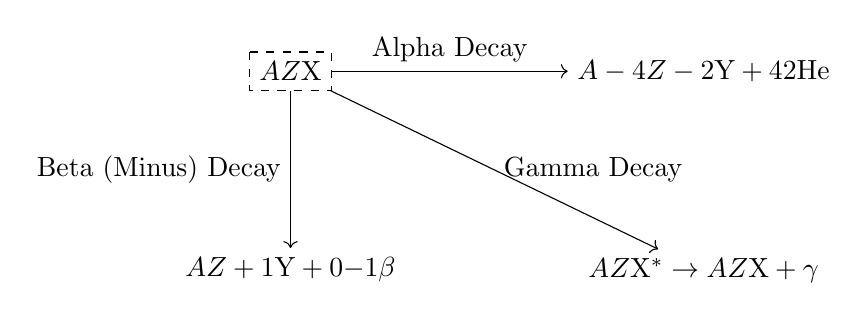
\begin{tikzpicture}[node distance=2cm, auto]

			% Alpha Decay
			\node (start) at (0,0) {$\prescript{A}{Z}{\mathrm{X}}$};
			\node (alpha) [right=3cm of start] {$\prescript{A-4}{Z-2}{\mathrm{Y}} + \prescript{4}{2}{\mathrm{He}}$};
			\draw[->] (start) -- node[above] {Alpha Decay} (alpha);

			% Beta Decay
			\node (beta) [below=2cm of start] {$\prescript{A}{Z+1}{\mathrm{Y}} + \prescript{0}{-1}{\beta}$};
			\draw[->] (start) -- node[left] {Beta (Minus) Decay} (beta);

			% Gamma Decay
			\node (gamma) [below=2cm of alpha] {$\prescript{A}{Z}{\mathrm{X^*}} \rightarrow \prescript{A}{Z}{\mathrm{X}} + \gamma$};
			\draw[->] (start) -- node[right] {Gamma Decay} (gamma);

			% Add a box around the initial nucleus
			\draw[dashed] (start.north west) rectangle (start.south east);


		\end{tikzpicture}
	\end{center}
}

\dfn{Alpha Decay}{

	\textbf{Alpha decay} is the most common nuclear decay process. \\
	Alpha decay is most common in nuclei with atomic number greater than 82 (the highest binding energy per nuclei).

}

\dfn{Binding Energy per Nucleon}{

	\[
		\Delta E = \Delta m c^2
	\]

	\[
		\Delta E = M_{Z,A} - \left( M_{Z-2} + M_{2, \alpha} \right) c^2 > 0
	\]

	\[
		\text{If } \Delta E > 0 \quad \Rightarrow \quad \text{Decay Occurs}
	\]

	\[
		\text{If } \Delta E < 0 \quad \Rightarrow \quad \text{Stable}
	\]
	\centering
	\includegraphics[width=0.5\textwidth]{BEPN.png} % Adjust the width as needed
	\par\vspace{1em} % Adds a small space after the image

}

\dfn{Beta Decay}{

	\textbf{Beta decay} occurs when a nucleus emits or absorbs a neutron. \\
	Beta decay is very common in nuclei with atomic number less than 82.


}

\dfn{Gamma Decay}{
	\textbf{Gamma decay} occurs when a nucleus emits or absorbs a photon. \\
	Gamma decay is rare, but it can occur in high-energy nuclei.

	Photons of electromagnetic radiation that carry away excess energy when nuclei make $\gamma$ decay.

}
\section{19.6 - Nuclear Fusion}

\dfn{Origin of elements}{
	\textbf{Fusion of elements} involves 2 nuclei of very low A amalgamating to a form a more stable nucleus. \\
	Getting the A value nearer to 56 (the highest Binding Energy per nucleon).
}

\nt{Hubbles observaions of red shift in further galaxies and knowledge of fusion leads us to predict the existence of a singularity at the start of the current universe. What came before this is not known, but it is believed to be a singularity of the same type as the one at the end of the universe.\\
	\textbf{The Steady State model } states that the densigty of the expanding universe should remain constant. As the universe expands, the density of matter stays the same as more matter is created.
}

\dfn{Initial Events of Big Bang}{
	\begin{align*}
		{}^1_0 \text{n}                   & \rightarrow {}^1_1 \text{H} + e^- + \bar{\nu}_e \\
		{}^1_1 \text{H} + \nu_e           & \rightarrow {}^1_0 \text{n} + e^+               \\
		{}^1_1 \text{H} + {}^1_0 \text{n} & \rightarrow {}^2_1 \text{H} + \gamma            \\
		e^+ + e^-                         & \rightarrow \gamma + \gamma
	\end{align*}


	\begin{center}
		\textbf{Then}
	\end{center}

	\begin{align*}
		{}^1_1 \text{H} + {}^1_0 \text{n}  & \rightarrow {}^2_1 \text{H} + \gamma           \\
		{}^2_1 \text{H} + {}^2_1 \text{H}  & \rightarrow {}^3_2 \text{He} + {}^1_0 \text{n} \\
		{}^3_2 \text{He} + {}^1_0 \text{n} & \rightarrow {}^4_2 \text{He} + \gamma          \\
		{}^3_2 \text{He} + {}^1_1 \text{H} & \rightarrow {}^4_2 \text{He}
	\end{align*}
	\begin{center}
		\textbf{Helium 3 (werid particle due to its quantum behavior) and helium 4 are created $1/10$ of the time}
	\end{center}
}

\nt{The fusion of 1 gram  deuterium and helium 3 gives about 350 billion joules of energy. Reason for which we are trying to reproduce fission on earth}



\thm{Clusters}
{
	Ripples in the helium and tritium gas clouds form denser regions, which group further due to gravity $\rightarrow$ hydrogen burn $\rightarrow$ HE is formed in a star cycle of reactions (proton-proton cycle) and heavier elements move
	towards the center. Outer portions do proton-proton burn, inner denser portions of the start do helium burn.$\rightarrow$ Helium 4's combine to make Beryllium $^8_4\text{Be}$. Beryllium and Helium combine to make carbon 12 $^{12}_6\text{C}$. $\rightarrow$ CARBON CYCLE occurs as $^{12}_6\text{C}$ is the catalyst.
	By adding helium $^4_2\text{He}$ to all the elements in the dense cores, all the elements up to iron $^{56}_{26}\text{Fe}$ formed, and then stopped due to it having the highest binding energy per nucleon.
}

\thm{After Iron}{
	A 14 particle collision is needed to make elements after Iron, which is very unlikely.
	\[
		^{56}_{26}\text{Fe} + 13 ^1_0\text{n} \rightarrow ^{69}_{26}\text{Co} + e
	\]
}

\nt{Fusion only gets us 26 elements (in stars).}

\pagebreak

\chapter{Chemical Structures}

\section{Drawing Lewis Dot Structures}

Lewis dot structures are diagrams that show the bonding between atoms of a molecule and the lone pairs of electrons that may exist in the molecule. Here's a step-by-step guide on how to draw Lewis dot structures:

\subsection{Steps to Draw a Lewis Dot Structure}

1. \textbf{Count the Valence Electrons:}
Find the total number of valence electrons in the molecule by adding up the valence electrons of all atoms.

2. \textbf{Arrange the Atoms:}
Write the atoms in the molecule with the least electronegative atom as the central atom (except for hydrogen, which is always terminal).

3. \textbf{Form Bonds Between Atoms:}
Connect the atoms with single bonds. Each bond represents a pair of shared electrons.

4. \textbf{Distribute Remaining Electrons:}
Distribute the remaining valence electrons as lone pairs around the atoms to satisfy their octet (or duet for hydrogen).

5. \textbf{Complete Octets:}
Make sure that each atom (except hydrogen) has 8 electrons around it by sharing additional pairs of electrons to form double or triple bonds if necessary.

6. \textbf{Check Formal Charges:}
If necessary, minimize formal charges to ensure that the most stable structure is drawn.

\subsection{Example Structures}

\subsubsection{Water (H\textsubscript{2}O)}

The water molecule consists of two hydrogen atoms and one oxygen atom. Oxygen has 6 valence electrons, and each hydrogen has 1 valence electron, making a total of 8 valence electrons.

The Lewis structure is drawn as follows:
\[
	\chemfig{H-[:30]O-[:-30]H}
\]

In this structure, the oxygen atom forms single bonds with each hydrogen atom and has two lone pairs of electrons.

\subsubsection{Carbon Dioxide (CO\textsubscript{2})}

The carbon dioxide molecule consists of one carbon atom and two oxygen atoms. Carbon has 4 valence electrons, and each oxygen has 6, making a total of 16 valence electrons.

The Lewis structure is drawn as follows:
\[
	\chemfig{O=[:30]C=[:-30]O}
\]

In this structure, the carbon atom forms double bonds with each oxygen atom, and each oxygen has two lone pairs of electrons.

\pagebreak

\section{Common Molecular Shapes}

\subsection{2 Electron Pairs - Linear - AX\textsubscript{2}}
In molecules with 2 bonding pairs and no lone pairs, the atoms are arranged in a straight line, resulting in a bond angle of 180$^\circ$.
\begin{center}
	\chemfig{A-[:180]B}
\end{center}

\subsection{3 Electron Pairs - Trigonal Planar - AX\textsubscript{3}}
When there are 3 bonding pairs and no lone pairs, the atoms are positioned around the central atom in a single plane, forming a bond angle of 120$^\circ$.
\begin{center}
	\chemfig{A(-[:90]B)(-[:210]C)(-[:330]D)}
\end{center}

\subsubsection{3 Electron Pairs (1 Lone Pair) - Bent - AX\textsubscript{2}E}
If there are 2 bonding pairs and 1 lone pair, the lone pair causes a repulsion that slightly decreases the bond angle to less than 120$^\circ$.
\begin{center}
	\chemfig{A(-[:90]B)(-[:210]C)}
\end{center}

\subsection{4 Electron Pairs - Tetrahedral - AX\textsubscript{4}}
For 4 bonding pairs and no lone pairs, the atoms are arranged in a tetrahedral shape with bond angles of 109.5$^\circ$.
\begin{center}
	\chemfig{A(-[:90]B)(-[:210]C)(-[:330]D)(-[:0]E)}
\end{center}

\subsubsection{4 Electron Pairs (1 Lone Pair) - Trigonal Pyramidal - AX\textsubscript{3}E}
When there are 3 bonding pairs and 1 lone pair, the structure becomes trigonal pyramidal, and the lone pair repulsion decreases the bond angles to slightly less than 109.5$^\circ$.
\begin{center}
	\chemfig{A(-[:0]B)(-[:210]C)(-[:330]D)}
\end{center}

\subsubsection{4 Electron Pairs (2 Lone Pairs) - Bent AX\textsubscript{2}E\textsubscript{2}}
With 2 bonding pairs and 2 lone pairs, the shape is bent, with bond angles further reduced to less than 109.5$^\circ$.
\begin{center}
	\chemfig{A(-[:90]B)(-[:210]C)}
\end{center}

\subsection{5 Electron Pairs - Trigonal Bipyramidal}
For 5 bonding pairs and no lone pairs, the shape is trigonal bipyramidal, with bond angles of 90$^\circ$ (axial) and 120$^\circ$ (equatorial).
\begin{center}
	\chemfig{A(-[:90]B)(-[:150]C)(-[:230]D)(-[:270]E)(-[:30]F)}
\end{center}

\subsubsection{5 Electron Pairs (1 Lone Pair) - Seesaw}
With 4 bonding pairs and 1 lone pair, the structure becomes a seesaw, and the bond angles are slightly adjusted due to lone pair repulsion.
\begin{center}
	\chemfig{A(-[:90]B)(-[:150]C)(-[:230]D)(-[:270]E)}
\end{center}

\subsubsection{5 Electron Pairs (2 Lone Pairs) - T-Shaped}
When there are 3 bonding pairs and 2 lone pairs, the shape is T-shaped, with bond angles around 90$^\circ$.
\begin{center}
	\chemfig{A(-[:90]B)(-[:180]C)(-[:270]D)}
\end{center}

\subsubsection{5 Electron Pairs (3 Lone Pairs) - Linear}
With 2 bonding pairs and 3 lone pairs, the shape reverts to linear with a bond angle of 180$^\circ$.
\begin{center}
	\chemfig{A-[:180]B}
\end{center}

\subsection{6 Electron Pairs - Octahedral}
In a molecule with 6 bonding pairs and no lone pairs, the atoms are arranged in an octahedral shape with bond angles of 90$^\circ$.
\begin{center}
	\chemfig{A(-[:90]B)(-[:150]C)(-[:210]D)(-[:270]E)(-[:30]F)(-[:330]G)}
\end{center}

\subsubsection{6 Electron Pairs (1 Lone Pair) - Square Pyramidal}
For 5 bonding pairs and 1 lone pair, the structure is square pyramidal, with slightly less than 90$^\circ$ bond angles due to lone pair repulsion.
\begin{center}
	\chemfig{A(-[:90]B)(-[:150]C)(-[:210]D)(-[:270]E)(-[:30]F)}
\end{center}

\subsubsection{6 Electron Pairs (2 Lone Pairs) - Square Planar}
With 4 bonding pairs and 2 lone pairs, the molecule is square planar, maintaining bond angles of 90$^\circ$.
\begin{center}
	\chemfig{A(-[:90]B)(-[:150]C)(-[:210]D)(-[:270]E)}
\end{center}

\subsection{7 Electron Pairs - Pentagonal Bipyramidal}
For 7 bonding pairs and no lone pairs, the atoms are arranged in a pentagonal bipyramidal shape with bond angles of 72$^\circ$ (within the pentagon) and 90$^\circ$ (between axial and equatorial positions).
\begin{center}
	\chemfig{A(-[:90]B)(-[:54]C)(-[:18]D)(-[:306]E)(-[:270]F)(-[:234]G)(-[:198]H)}
\end{center}

\section{Dipole Moment}

The dipole moment is a measure of the separation of positive and negative charges in a molecule. It is a vector quantity, possessing both magnitude and direction. Molecules with polar bonds may have a net dipole moment if their molecular geometry does not cancel out the individual bond dipoles. The dipole moment influences many physical properties such as solubility, boiling point, and reactivity.

\subsection{Examples}

\subsubsection{Carbon Tetrachloride (CCl$_4$)}

Carbon tetrachloride is a symmetric molecule where the four C--Cl bonds are directed towards the corners of a tetrahedron. Although each C--Cl bond is polar due to the difference in electronegativity between carbon and chlorine, the symmetry of the molecule causes the bond dipoles to cancel out, resulting in a net dipole moment of zero.

\begin{figure}[h]
	\centering
	\begin{tikzpicture}
		% Draw the carbon atom at the center
		\node (C) at (0,0) {C};
		% Positions for the four chlorine atoms
		\node (Cl1) at (1.5,0) {Cl};
		\node (Cl2) at (-1.5,0) {Cl};
		\node (Cl3) at (0,1.5) {Cl};
		\node (Cl4) at (0,-1.5) {Cl};
		% Draw bonds
		\draw (C) -- (Cl1);
		\draw (C) -- (Cl2);
		\draw (C) -- (Cl3);
		\draw (C) -- (Cl4);
		% Indicate dipole moments
		\draw[->,red,thick] (C) -- ++(0.75,0);
		\draw[->,red,thick] (C) -- ++(-0.75,0);
		\draw[->,red,thick] (C) -- ++(0,0.75);
		\draw[->,red,thick] (C) -- ++(0,-0.75);
		% Label the dipoles
		\node[red] at (0.9,0.2) {$\mu$};
		\node[red] at (-0.9,0.2) {$\mu$};
		\node[red] at (0.2,0.9) {$\mu$};
		\node[red] at (0.2,-0.9) {$\mu$};
	\end{tikzpicture}
	\caption{Molecular structure of CCl$_4$ showing bond dipoles cancelling out.}
\end{figure}

\subsubsection{Chloroform (CHCl$_3$)}

Chloroform has a similar tetrahedral geometry as carbon tetrachloride but with one hydrogen atom replacing one of the chlorine atoms. This asymmetry results in bond dipoles that do not completely cancel out, giving chloroform a net dipole moment.

\begin{figure}[h]
	\centering
	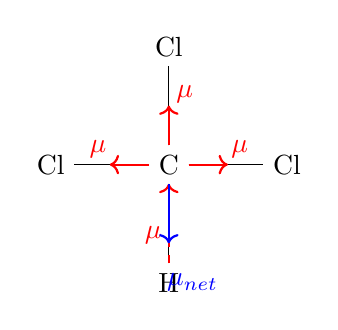
\begin{tikzpicture}
		% Draw the carbon atom at the center
		\node (C) at (0,0) {C};
		% Positions for the three chlorine atoms and one hydrogen atom
		\node (Cl1) at (1.5,0) {Cl};
		\node (Cl2) at (-1.5,0) {Cl};
		\node (Cl3) at (0,1.5) {Cl};
		\node (H) at (0,-1.5) {H};
		% Draw bonds
		\draw (C) -- (Cl1);
		\draw (C) -- (Cl2);
		\draw (C) -- (Cl3);
		\draw (C) -- (H);
		% Indicate dipole moments
		\draw[->,red,thick] (C) -- ++(0.75,0);
		\draw[->,red,thick] (C) -- ++(-0.75,0);
		\draw[->,red,thick] (C) -- ++(0,0.75);
		\draw[->,red,thick,dashed] (H) -- (C);
		% Label the dipoles
		\node[red] at (0.9,0.2) {$\mu$};
		\node[red] at (-0.9,0.2) {$\mu$};
		\node[red] at (0.2,0.9) {$\mu$};
		\node[red] at (-0.2,-0.9) {$\mu$};
		% Indicate net dipole moment
		\draw[->,blue,thick] (C) -- ++(0,-1);
		\node[blue] at (0.3,-1.5) {$\mu_{net}$};
	\end{tikzpicture}
	\caption{Molecular structure of CHCl$_3$ showing bond dipoles and net dipole moment.}
\end{figure}

\chapter{Quantum Mechanics}

\section{Electromagnetic Fields in Light}

Electromagnetic (EM) waves are composed of electric and magnetic fields oscillating perpendicularly to each other and to the direction of wave propagation. Light is an example of an EM wave, and it travels at the speed of light in a vacuum.

The electric field (\(E\)) and magnetic field (\(B\)) are perpendicular to each other, and both are perpendicular to the direction of wave propagation. Below is a simplified representation of an electromagnetic wave:

\begin{center}
	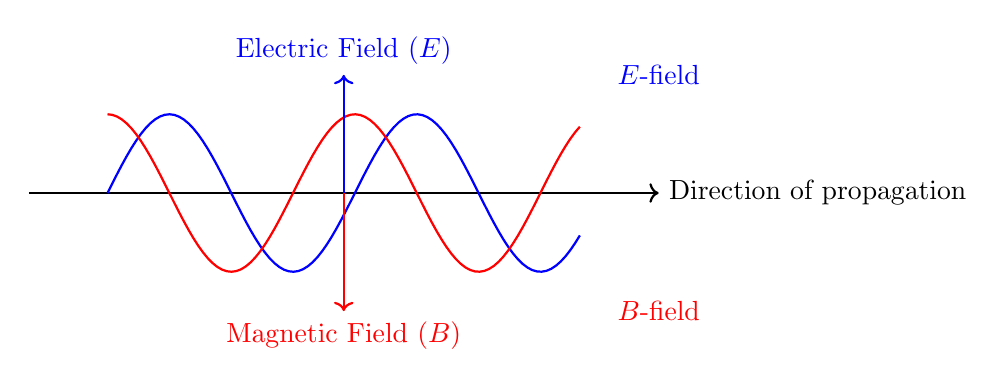
\begin{tikzpicture}[scale=1.0]
		% Wave propagation direction
		\draw[->, thick] (-1, 0) -- (7, 0) node[right] {Direction of propagation};

		% Electric field wave (in blue)
		\draw[blue, thick, domain=0:6, variable=\x, samples=100]
		plot ({\x}, {sin(2 * \x r)});
		\node[blue] at (7, 1.5) {$E$-field};

		% Magnetic field wave (in red)
		\draw[red, thick, domain=0:6, variable=\x, samples=100]
		plot ({\x}, {cos(2 * \x r)});
		\node[red] at (7, -1.5) {$B$-field};

		% Labels
		\draw[->, thick, blue] (3, 0) -- (3, 1.5) node[above] {Electric Field ($E$)};
		\draw[->, thick, red] (3, 0) -- (3, -1.5) node[below] {Magnetic Field ($B$)};
	\end{tikzpicture}
\end{center}

In this diagram, the electric field (\(E\)) oscillates in one plane, while the magnetic field (\(B\)) oscillates in a perpendicular plane. Both fields are sinusoidal and propagate together in the direction shown.

\section{The Wave Equation: \(c = f \lambda\)}

The relationship between the speed of light (\(c\)), the frequency (\(f\)), and the wavelength (\(\lambda\)) of an electromagnetic wave is given by the equation:
\[
	c = f \lambda
\]
where:
\begin{itemize}
	\item \(c\) is the speed of light in a vacuum, approximately \(3 \times 10^8\) m/s,
	\item \(f\) is the frequency of the wave (in Hz),
	\item \(\lambda\) is the wavelength of the wave (in meters).
\end{itemize}

This equation shows that the speed of light is the product of its frequency and wavelength. As the frequency of a wave increases, its wavelength decreases, and vice versa.

\section{The Electromagnetic Spectrum}

The electromagnetic spectrum encompasses all types of electromagnetic radiation, ranging from low-frequency radio waves to high-frequency gamma rays. Below is a diagram showing the range of the spectrum:

\begin{center}
	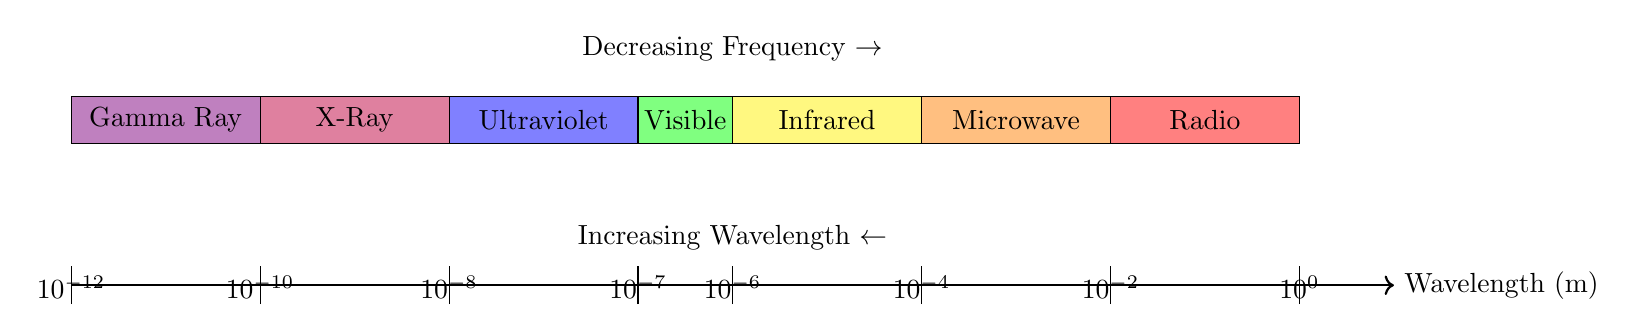
\begin{tikzpicture}[scale=1.2]
		% Spectrum axis

		% Spectrum sections (flipped)
		\draw[fill=violet!50] (0, 0.5) rectangle (2, 1) node[midway] {Gamma Ray};
		\draw[fill=purple!50] (2, 0.5) rectangle (4, 1) node[midway] {X-Ray};
		\draw[fill=blue!50] (4, 0.5) rectangle (6, 1) node[midway] {Ultraviolet};
		\draw[fill=green!50] (6, 0.5) rectangle (7, 1) node[midway] {Visible};
		\draw[fill=yellow!50] (7, 0.5) rectangle (9, 1) node[midway] {Infrared};
		\draw[fill=orange!50] (9, 0.5) rectangle (11, 1) node[midway] {Microwave};
		\draw[fill=red!50] (11, 0.5) rectangle (13, 1) node[midway] {Radio};

		% Labels for increasing frequency and decreasing wavelength
		\node at (7, 1.5) {Decreasing Frequency $\rightarrow$};
		\node at (7, -0.5) {Increasing Wavelength $\leftarrow$};

		% Wavelength ticks
		\draw[thick, ->] (0, -1) -- (14, -1) node[right] {Wavelength (m)};
		\draw (0, -1.2) -- (0, -0.8) node[below] {$10^{-12}$};
		\draw (2, -1.2) -- (2, -0.8) node[below] {$10^{-10}$};
		\draw (4, -1.2) -- (4, -0.8) node[below] {$10^{-8}$};
		\draw (6, -1.2) -- (6, -0.8) node[below] {$10^{-7}$};
		\draw (7, -1.2) -- (7, -0.8) node[below] {$10^{-6}$};
		\draw (9, -1.2) -- (9, -0.8) node[below] {$10^{-4}$};
		\draw (11, -1.2) -- (11, -0.8) node[below] {$10^{-2}$};
		\draw (13, -1.2) -- (13, -0.8) node[below] {$10^{0}$};
	\end{tikzpicture}
\end{center}

The electromagnetic spectrum ranges from long-wavelength, low-frequency waves like radio waves to short-wavelength, high-frequency waves like gamma rays. Visible light is a small portion of the spectrum, spanning from approximately 400 nm (violet) to 700 nm (red) in wavelength.

\section{Absorption Spectrum of Elements}

The absorption spectrum of an element is a unique pattern of dark lines or bands that appear when white light passes through a gas or vapor composed of the element. These dark lines correspond to specific wavelengths of light that have been absorbed by the element's atoms. Understanding absorption spectra is crucial in fields like astronomy and spectroscopy, as they allow scientists to identify elements in stars and distant galaxies.

\subsection{How Absorption Spectra Work}

When white light (which contains all visible wavelengths) passes through a sample of an element in its gaseous state, the electrons in the atoms of that element absorb specific amounts of energy. This energy corresponds to the difference between specific energy levels or orbits of the electrons.

When electrons absorb this energy, they jump from a lower energy level to a higher energy level, creating an absorption event. Each element has a unique set of energy levels, so the wavelengths absorbed (or "dark lines" in the spectrum) are also unique to each element. These dark lines are referred to as \textbf{absorption lines}.

\subsection{Relationship to Emission Spectrum}

The absorption spectrum is closely related to the \textbf{emission spectrum} of an element. When an electron drops from a higher energy level to a lower one, it emits light at a wavelength corresponding to the energy difference between these levels. In contrast, the absorption spectrum is formed when electrons move from lower to higher energy levels by absorbing light.

The emission lines and absorption lines occur at the same wavelengths for any given element, but they appear differently in the spectra:
\begin{itemize}
	\item \textbf{Emission Spectrum}: Bright lines on a dark background, representing wavelengths emitted by electrons falling to lower energy levels.
	\item \textbf{Absorption Spectrum}: Dark lines on a bright (continuous) background, representing wavelengths absorbed by electrons jumping to higher energy levels.
\end{itemize}

\subsection{Example: Hydrogen Absorption Spectrum}

The hydrogen atom, for example, has a simple absorption spectrum. It consists of a series of dark lines in the visible region, corresponding to the specific wavelengths absorbed by electrons as they move to higher energy levels. The Balmer series is a well-known part of hydrogen's absorption spectrum, with lines appearing in the visible light range.

Below is a simplified representation of the absorption spectrum of hydrogen:
\[
	\text{--- --- --- --- ---}
\]
The dark lines represent wavelengths absorbed by the hydrogen atoms.

\subsection{Applications of Absorption Spectra}

Absorption spectra are used in a variety of scientific fields to:
\begin{itemize}
	\item Identify elements present in stars and distant astronomical objects.
	\item Determine the chemical composition of substances.
	\item Study the energy levels and quantum mechanics of atoms and molecules.
\end{itemize}

Since each element has a unique absorption spectrum, this technique allows scientists to detect and analyze the presence of different elements based on the pattern of dark lines that appear in a spectrum.

\begin{center}
	
\begin{tikzpicture}[scale=1.0]
		% Continuous spectrum
		\shade[left color=white, right color=black] (0, 0) rectangle (10, 0.5);
		% Absorption lines
		\draw[very thick, white] (2, 0) -- (2, 0.5);
		\draw[very thick, white] (4, 0) -- (4, 0.5);
		\draw[very thick, white] (6, 0) -- (6, 0.5);
		\draw[very thick, white] (8, 0) -- (8, 0.5);
	\end{tikzpicture}
\end{center}

In this diagram, the gradient from white to black represents the continuous spectrum of light, while the vertical white lines represent absorption lines where specific wavelengths are absorbed by the element.

\section{Rydberg Equations and Emission Spectra}

The planetary model of the atom pictures electrons orbiting the nucleus in the way that planets orbit the sun. Bohr used the planetary model to develop the first reasonable theory of hydrogen, the simplest atom. Atomic and molecular spectra are quantized, with hydrogen spectrum wavelengths given by the formula:
\[
	\frac{1}{\lambda} = R Z^2 \left( \frac{1}{n_f^2} - \frac{1}{n_i^2} \right),
\]
where $\lambda$ is the wavelength of the emitted EM radiation and $R$ is the Rydberg constant, which has the value
\[
	R = 1.097 \times 10^7 \text{ m}^{-1}.
\]
The constants $n_i$ and $n_f$ are positive integers, and $n_i$ must be greater than $n_f$.

Bohr correctly proposed that the energy and radii of the orbits of electrons in atoms are quantized, with energy for transitions between orbits given by
\[
	\Delta E = hf = E_i - E_f, \tag{30.3.22}
\]
where $\Delta E$ is the change in energy between the initial and final orbits and $hf$ is the energy of an absorbed or emitted photon. It is useful to plot orbital energies on a vertical graph called an energy-level diagram.

Bohr proposed that the allowed orbits are circular and must have quantized orbital angular momentum given by
\[
	L = m_e v_n r_n = n \frac{h}{2 \pi} \quad (n = 1, 2, 3, \ldots),
\]
where $L$ is the angular momentum, $r_n$ is the radius of the $n$th orbit, and $h$ is Planck's constant. For all one-electron (hydrogen-like) atoms, the radius of an orbit is given by
\[
	r_n = \frac{n^2}{Z} a_B \quad \text{(allowed orbits } n = 1, 2, 3, \ldots),
\]
$Z$ is the atomic number of an element (the number of electrons it has when neutral) and $a_B$ is defined to be the Bohr radius, which is
\[
	a_B = \frac{h^2}{4 \pi^2 m_e k e^2} = 0.529 \times 10^{-10} \text{ m}.
\]

Furthermore, the energies of hydrogen-like atoms are given by
\[
	E_n = -\frac{Z^2}{n^2} E_0 \quad (n = 1, 2, 3, \ldots),
\]
where $E_0$ is the ground-state energy and is given by
\[
	E_0 = \frac{2 \pi^2 m_e k^2 e^4}{h^2} = 13.6 \text{ eV}.
\]
Thus, for hydrogen,
\[
	E_n = -\frac{13.6 \text{ eV}}{n^2} \quad (n = 1, 2, 3, \ldots).
\]

The Bohr Theory gives accurate values for the energy levels in hydrogen-like atoms, but it has been improved upon in several respects.

\subsection{Applications of Rydberg Equation}

The Rydberg equation is not only crucial for predicting the emission spectrum of hydrogen but also for understanding other one-electron systems like He$^+$, Li$^{2+}$, and so forth. By studying the emission spectra of various elements, scientists can gain insights into the structure of atoms and the quantized nature of their energy levels. The emission spectra are also used in astrophysics to identify the elements present in distant stars and galaxies by comparing observed spectral lines with known values.

\section{Max Planck’s 1900 Theory and the Relationship $E = h\nu$}

In the early 1900s, Max Planck introduced a revolutionary concept that laid the foundation for quantum mechanics. To address the problem of blackbody radiation, Planck proposed that electromagnetic energy could only be emitted or absorbed in discrete units, or "quanta." This concept was a significant departure from classical physics and led to the development of the famous relationship:

\[
	E = h \nu,
\]

where:
\begin{itemize}
	\item $E$ is the energy of a quantum (or photon) of electromagnetic radiation.
	\item $h$ is Planck’s constant, with a value of approximately $6.626 \times 10^{-34} \, \text{Js}$.
	\item $\nu$ (or $f$) is the frequency of the electromagnetic radiation.
\end{itemize}

\subsection{The Blackbody Radiation Problem}

Classical physics predicted that a blackbody (an idealized physical body that absorbs all incident electromagnetic radiation) would emit radiation with an intensity that increases infinitely as the wavelength decreases (known as the “ultraviolet catastrophe”). However, experimental observations showed that the intensity reaches a peak and then drops off at shorter wavelengths. This discrepancy between theory and experiment led to the need for a new understanding of how radiation is emitted.

\subsection{Planck's Solution: Quantization of Energy}

Planck hypothesized that the energy emitted by a blackbody could only take on discrete values, rather than being continuous. He proposed that the energy of each quantum of radiation is proportional to its frequency, leading to the equation:
\[
	E = h \nu.
\]

This assumption meant that electromagnetic radiation is quantized and that the energy levels are spaced in multiples of $h \nu$. In essence, energy could only be emitted or absorbed in “packets” or quanta, not as a continuous wave.

\subsection{Implications of Planck's Theory}

Planck’s theory successfully explained the blackbody radiation spectrum, and the constant $h$, later known as Planck's constant, became a fundamental constant in quantum mechanics. This idea of quantization was groundbreaking because it introduced the concept that energy is not infinitely divisible, contradicting the classical wave theory of light.

The relationship $E = h \nu$ implies that higher frequency (shorter wavelength) radiation has more energy per photon. This paved the way for the development of quantum theory and influenced subsequent discoveries, including:
\begin{itemize}
	\item \textbf{Photoelectric Effect}: Albert Einstein used Planck’s concept to explain the photoelectric effect in 1905, showing that light can eject electrons from a material if the frequency is above a certain threshold. This provided further evidence of the particle-like behavior of light.
	\item \textbf{Wave-Particle Duality}: Planck’s work suggested that light exhibits both wave-like and particle-like properties, an idea that became central to quantum mechanics.
	\item \textbf{Quantum Energy Levels}: The concept of quantized energy levels led to the understanding of atomic structure and the development of quantum mechanical models, where electrons occupy discrete energy states around the nucleus.
\end{itemize}

\subsection{Applications and Further Developments}

Planck’s relationship, $E = h \nu$, has vast implications in various fields of physics and chemistry. It underpins the understanding of atomic spectra, molecular vibrations, and electronic transitions. It also plays a crucial role in technologies such as lasers, semiconductors, and quantum computing.

Overall, Planck’s introduction of the quantization of energy marked the beginning of a new era in physics, laying the groundwork for the development of quantum mechanics and fundamentally changing our understanding of the physical world.

\subsection{Quantized Emission Spectra}


\begin{center}
	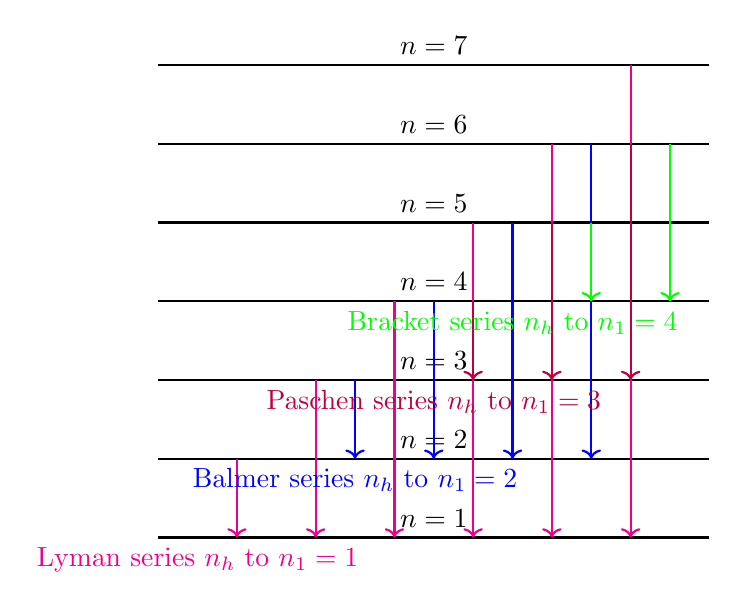
\begin{tikzpicture}

		% Define the energy levels
		\draw[thick] (0,0) -- (7,0) node[pos=0.5, above] {$n=1$};
		\draw[thick] (0,1) -- (7,1) node[pos=0.5, above] {$n=2$};
		\draw[thick] (0,2) -- (7,2) node[pos=0.5, above] {$n=3$};
		\draw[thick] (0,3) -- (7,3) node[pos=0.5, above] {$n=4$};
		\draw[thick] (0,4) -- (7,4) node[pos=0.5, above] {$n=5$};
		\draw[thick] (0,5) -- (7,5) node[pos=0.5, above] {$n=6$};
		\draw[thick] (0,6) -- (7,6) node[pos=0.5, above] {$n=7$};

		% Lyman series (n_h to n_1=1)
		\foreach \x in {1,2,3,4,5,6} {
				\draw[thick, magenta, ->] (\x, \x) -- (\x, 0);
			}
		\node[magenta, below] at (0.5,0) {Lyman series $n_h$ to $n_1=1$};

		% Balmer series (n_h to n_1=2)
		\foreach \x in {2,3,4,5} {
				\draw[thick, blue, ->] (\x+0.5, \x) -- (\x+0.5, 1);
			}
		\node[blue, below] at (2.5,1) {Balmer series $n_h$ to $n_1=2$};

		% Paschen series (n_h to n_1=3)
		\foreach \x in {3,4,5} {
				\draw[thick, purple, ->] (\x+1, \x) -- (\x+1, 2);
			}
		\node[purple, below] at (3.5,2) {Paschen series $n_h$ to $n_1=3$};

		% Bracket series (n_h to n_1=4)
		\foreach \x in {4,5} {
				\draw[thick, green, ->] (\x+1.5, \x) -- (\x+1.5, 3);
			}
		\node[green, below] at (4.5,3) {Bracket series $n_h$ to $n_1=4$};

	\end{tikzpicture}

\end{center}

\section{The Photoelectric Effect}

The photoelectric effect is a phenomenon in which electrons are ejected from the surface of a material (usually a metal) when it is exposed to light of sufficient frequency. The experimental observations of the photoelectric effect could not be explained by classical wave theory and led to the development of quantum theory. Albert Einstein provided the explanation for this effect in 1905 by extending Max Planck's concept of quantization of energy.

\subsection{Einstein’s Explanation}

According to Einstein, light consists of packets of energy called "photons," each with an energy $E$ given by:
\[
	E = h f,
\]
where:
\begin{itemize}
	\item $h$ is Planck’s constant ($6.626 \times 10^{-34} \, \text{Js}$).
	\item $f$ is the frequency of the incident light.
\end{itemize}

When a photon hits the surface of a material, its energy is transferred to an electron. If the photon's energy is greater than a certain minimum energy needed to free the electron (known as the \textbf{work function} $\Phi$ of the material), the electron is ejected from the surface.

\subsection{The Photoelectric Equation}

The maximum kinetic energy $E_{\text{max}}$ of the ejected electron is given by the equation:
\[
	E_{\text{max}} = h f - \Phi,
\]
where:
\begin{itemize}
	\item $E_{\text{max}}$ is the maximum kinetic energy of the ejected electron.
	\item $h f$ is the energy of the incident photon.
	\item $\Phi$ is the work function of the material, which is the minimum energy required to free an electron from the surface.
\end{itemize}

This equation implies that the kinetic energy of the ejected electron depends linearly on the frequency of the incident light, and there is a threshold frequency $f_{\text{threshold}}$ below which no electrons are ejected, regardless of the intensity of the light.

\subsection{Stopping Voltage and Kinetic Energy}

The kinetic energy of the ejected electrons can be measured experimentally using a stopping voltage $V_s$. The stopping voltage is the voltage required to stop the ejected electrons from reaching the detector. The relationship between the stopping voltage and the kinetic energy is given by:
\[
	E_{\text{max}} = e V_s,
\]
where:
\begin{itemize}
	\item $e$ is the charge of the electron ($1.602 \times 10^{-19} \, \text{C}$).
	\item $V_s$ is the stopping voltage.
\end{itemize}

By measuring the stopping voltage for different frequencies of light, one can determine the work function $\Phi$ of the material and verify the linear relationship between $E_{\text{max}}$ and the frequency $f$ of the incident light.

\subsection{Significance of the Photoelectric Effect}

The photoelectric effect provided strong evidence for the quantization of light and supported the particle-like behavior of photons. This was a crucial step in the development of quantum mechanics. The effect also showed that the energy of ejected electrons is independent of the light’s intensity (which only affects the number of emitted electrons) and is instead solely dependent on the frequency of the incident light.

Applications of the photoelectric effect are found in various technologies, including photodetectors, solar cells, and photoelectron spectroscopy.

\subsection{Graph of Voltage vs. Kinetic Energy}

The photoelectric equation $E_{\text{max}} = h f - \Phi$ shows that the maximum kinetic energy of ejected electrons is linearly dependent on the frequency of the incident light. Experimentally, this relationship can be studied by plotting the stopping voltage $V_s$ (which is directly proportional to $E_{\text{max}}$) against the frequency $f$ of the incident light.


\begin{center}
	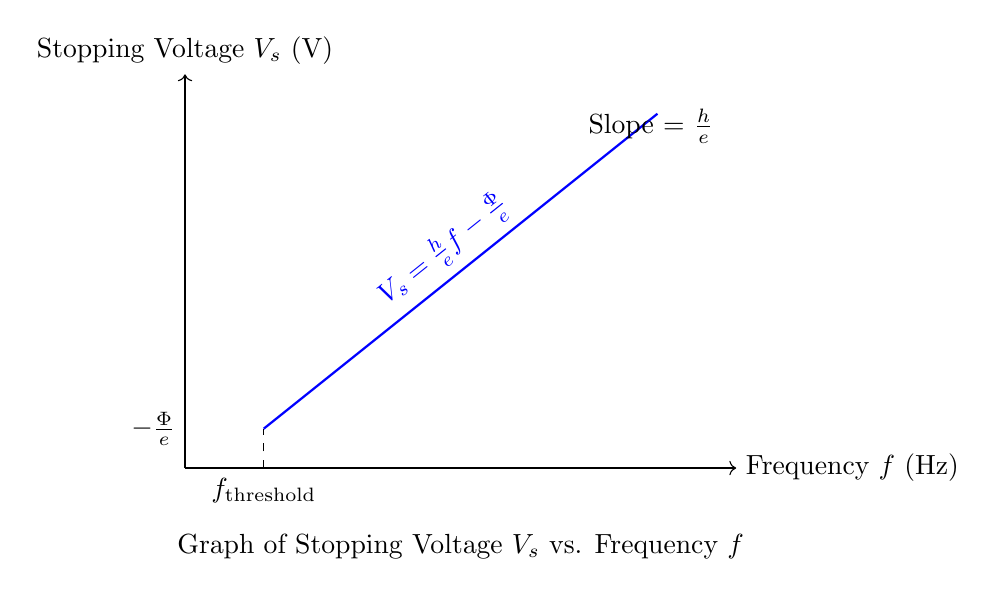
\begin{tikzpicture}
		% Axes
		\draw[->] (0,0) -- (7,0) node[right] {Frequency $f$ (Hz)};
		\draw[->] (0,0) -- (0,5) node[above] {Stopping Voltage $V_s$ (V)};

		% Line representing the photoelectric equation
		\draw[thick, blue] (1,0.5) -- (6,4.5) node[midway, above, sloped] {$V_s = \frac{h}{e}f - \frac{\Phi}{e}$};

		% Dots and line at threshold frequency
		\draw[dashed] (1,0) -- (1,0.5);
		\node[below] at (1,0) {$f_{\text{threshold}}$};

		% Labels for slope and intercept
		\node[above right] at (5,4) {Slope = $\frac{h}{e}$};
		\node[left] at (0,0.5) {$-\frac{\Phi}{e}$};

		% Label for graph
		\node at (3.5,-1) {Graph of Stopping Voltage $V_s$ vs. Frequency $f$};
	\end{tikzpicture}
\end{center}

\subsection{Explanation of the Graph}

The graph above represents the relationship between the stopping voltage $V_s$ and the frequency of the incident light $f$. The linear equation governing this relationship is:
\[
	V_s = \frac{h}{e} f - \frac{\Phi}{e},
\]
where:
\begin{itemize}
	\item $h$ is Planck’s constant.
	\item $e$ is the charge of an electron.
	\item $\Phi$ is the work function of the material.
\end{itemize}

In this graph:
\begin{itemize}
	\item The \textbf{slope} of the line is $\frac{h}{e}$. Since $h$ is Planck's constant and $e$ is a known constant (the electron charge), the slope provides a way to determine Planck's constant experimentally.
	\item The \textbf{y-intercept} is $-\frac{\Phi}{e}$, which corresponds to the work function of the material divided by the electron charge. This intercept is negative, as it represents the minimum energy needed to eject an electron.
	\item The point at which the line intersects the $f$-axis is the \textbf{threshold frequency} $f_{\text{threshold}}$. For frequencies below this value, no electrons are emitted because the photon's energy is insufficient to overcome the work function $\Phi$.
\end{itemize}

The linear nature of this graph is a direct consequence of the photoelectric effect and provides evidence for the quantization of energy in photons. By measuring the slope of this line, one can experimentally determine the value of Planck's constant $h$.

\section{Quantized Momentum of an Electron and Standing Waves in Orbits}

In the Bohr model of the atom, electrons are assumed to occupy discrete orbits around the nucleus. One of the key ideas is that the angular momentum of an electron in these orbits is quantized. Specifically, the angular momentum $L$ is given by:
\[
	L = n \hbar,
\]
where:
\begin{itemize}
	\item $n$ is a positive integer (the principal quantum number).
	\item $\hbar$ is the reduced Planck's constant ($\hbar = \frac{h}{2\pi}$).
\end{itemize}

This quantization arises because the electron behaves as a standing wave in its orbit. For a stable orbit, the circumference of the orbit must be an integer multiple of the electron's wavelength $\lambda$:
\[
	2 \pi r = n \lambda,
\]
where $r$ is the radius of the orbit.


\begin{center}
	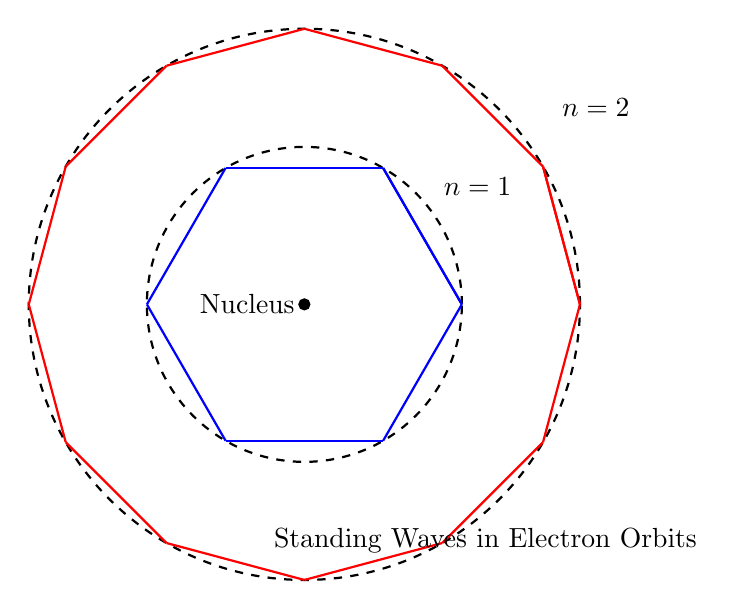
\begin{tikzpicture}
		% Nucleus
		\filldraw (0,0) circle (2pt) node[left] {Nucleus};

		% Orbits
		\draw[thick, dashed] (0,0) circle (2);
		\draw[thick, dashed] (0,0) circle (3.5);

		% Standing wave in the first orbit (n=1)
		\foreach \i in {0,60,...,360}
		\draw[thick, blue] ({2*cos(\i)},{2*sin(\i)}) -- ({2*cos(\i+60)},{2*sin(\i+60)});
		\node at (2.2,1.5) {$n=1$};

		% Standing wave in the second orbit (n=2)
		\foreach \i in {0,30,...,360}
		\draw[thick, red] ({3.5*cos(\i)},{3.5*sin(\i)}) -- ({3.5*cos(\i+30)},{3.5*sin(\i+30)});
		\node at (3.7,2.5) {$n=2$};

		% Labels
		\node at (2.3,-3) {Standing Waves in Electron Orbits};
	\end{tikzpicture}
\end{center}

\subsection{Standing Waves and Quantized Orbits}

For each allowed orbit, the electron’s de Broglie wavelength $\lambda$ fits perfectly into the circumference of the orbit, creating a standing wave. This condition ensures that only specific, quantized orbits are possible, corresponding to different values of $n$. The quantization of angular momentum restricts electrons to these stable orbits, preventing them from spiraling into the nucleus.

In the diagram:
\begin{itemize}
	\item The dashed circles represent possible orbits.
	\item The blue and red standing waves correspond to $n=1$ and $n=2$, respectively, showing how the electron’s wave fits into each orbit.
\end{itemize}

\subsection{Quantized Momentum of an Electron}

In the Bohr model of the atom, the momentum of an electron is quantized due to its wave-like nature. The electron behaves as a standing wave around the nucleus, and only certain orbits are allowed where the circumference of the orbit is an integer multiple of the electron's wavelength:
\[
	2 \pi r = n \lambda,
\]
where $r$ is the radius of the orbit, $n$ is a positive integer (the principal quantum number), and $\lambda$ is the de Broglie wavelength of the electron.

Since the de Broglie wavelength is related to momentum $p$ by:
\[
	\lambda = \frac{h}{p},
\]
the quantization condition becomes:
\[
	p = \frac{n \hbar}{r},
\]
where $\hbar = \frac{h}{2\pi}$. This shows that the electron’s momentum is quantized, allowing only specific values for each orbit.


\section{Heisenberg Uncertainty Principle}

The Heisenberg Uncertainty Principle is a fundamental concept in quantum mechanics, stating that it is impossible to simultaneously know the exact position and momentum of a particle. This principle arises due to the wave-like nature of particles at the quantum level. When attempting to measure one property (e.g., position), the wavefunction describing the particle's behavior is disturbed, leading to an increased uncertainty in the complementary property (e.g., momentum). This effect is a direct consequence of the properties of wavefunctions and Fourier transforms.

The principle is mathematically represented by the inequality:

\[
	\boxed{\Delta x \cdot \Delta p \geq \frac{\hbar}{4 \pi}}
\]

where:
- \(\Delta x\) is the uncertainty in position,
- \(\Delta p\) is the uncertainty in momentum,
- \(\hbar\) is  Planck's constant.

In other words, the product of the uncertainties in position and momentum can never be smaller than \(\frac{\hbar}{4 \pi}\).

A similar relationship exists between the uncertainties in energy and time, given by:

\[
	\boxed{\Delta E \cdot \Delta t \geq \frac{\hbar}{4 \pi}}
\]

where:
- \(\Delta E\) is the uncertainty in energy,
- \(\Delta t\) is the uncertainty in time.

This relationship arises because a particle's energy and the time over which it is measured are also complementary variables, meaning that a precise measurement of one leads to increased uncertainty in the other.

The Heisenberg Uncertainty Principle emphasizes the inherent limitations in our ability to measure certain pairs of physical properties simultaneously, reflecting the fundamental nature of quantum systems.


\section{Schrödinger's Equation and Atomic Orbitals}

Schrödinger's equation describes the behavior of quantum particles, particularly electrons in an atom. The time-independent form of the equation is:

\begin{equation}
	\hat{H}\psi = E\psi
\end{equation}

where $\hat{H}$ is the Hamiltonian operator, $\psi$ is the wavefunction, and $E$ is the energy of the system. In the context of atoms, solving this equation for electrons leads to quantized energy levels and wavefunctions, known as orbitals.

To reflect the symmetry of the atom, the wavefunction is expressed in spherical coordinates $(r, \theta, \phi)$ rather than Cartesian coordinates $(x, y, z)$. This simplifies the equation due to the spherical symmetry of the Coulomb potential around the nucleus, making it easier to solve for orbitals:

\begin{equation}
	\psi_{n,l,m_l}(r, \theta, \phi) = R(r)_{n,l}Y(\theta, \phi)_{l}
\end{equation}

Here, $R(r)$ describes the radial part, and $Y(\theta, \phi)$ represents the angular part of the wavefunction. The quantum numbers $n$, $l$, and $m_l$ arise from these solutions, defining the energy levels and shapes of atomic orbitals.

The quantum numbers have the following values and meanings:
\begin{itemize}
	\item The principal quantum number $n$ determines the electron's energy level and the shell in which the electron resides. It takes positive integer values: $n = 1, 2, 3, \dots$. The value of $n$ also correlates with the period (row) of the periodic table in which the element is found, and as $n$ increases, the electron's average distance from the nucleus and energy both increase.
	\item The azimuthal quantum number $l$ determines the shape of the orbital and the subshell, corresponding to the labels \(s\), \(p\), \(d\), and \(f\):
	      \begin{itemize}
		      \item $l = 0$: $s$-orbital (spherical)
		      \item $l = 1$: $p$-orbital (dumbbell-shaped)
		      \item $l = 2$: $d$-orbital (more complex shapes)
		      \item $l = 3$: $f$-orbital (even more complex shapes)
	      \end{itemize}
	      The possible values of $l$ range from $0$ to $n-1$ for a given energy level, defining which subshells are present within a shell.
	\item The magnetic quantum number $m_l$ defines the orientation of the orbital in space and takes integer values from $-l$ to $l$: $m_l = -l, -(l-1), \dots, 0, \dots, (l-1), l$. It specifies the number of orbitals within a subshell, such as the three orientations of the $p$-orbitals or the five orientations of the $d$-orbitals.
\end{itemize}
These quantum numbers collectively describe the unique characteristics of atomic orbitals, such as energy level, shape, orientation, and how they correspond to the organization of elements in the periodic table.
\begin{itemize}
	\item Total Nodes = $n-1$
	\item Total Angular Nodes = $l$
	\item Total Radial Nodes = $n-l-1$
\end{itemize}


\section{Energy Diagram for Atomic Orbitals}

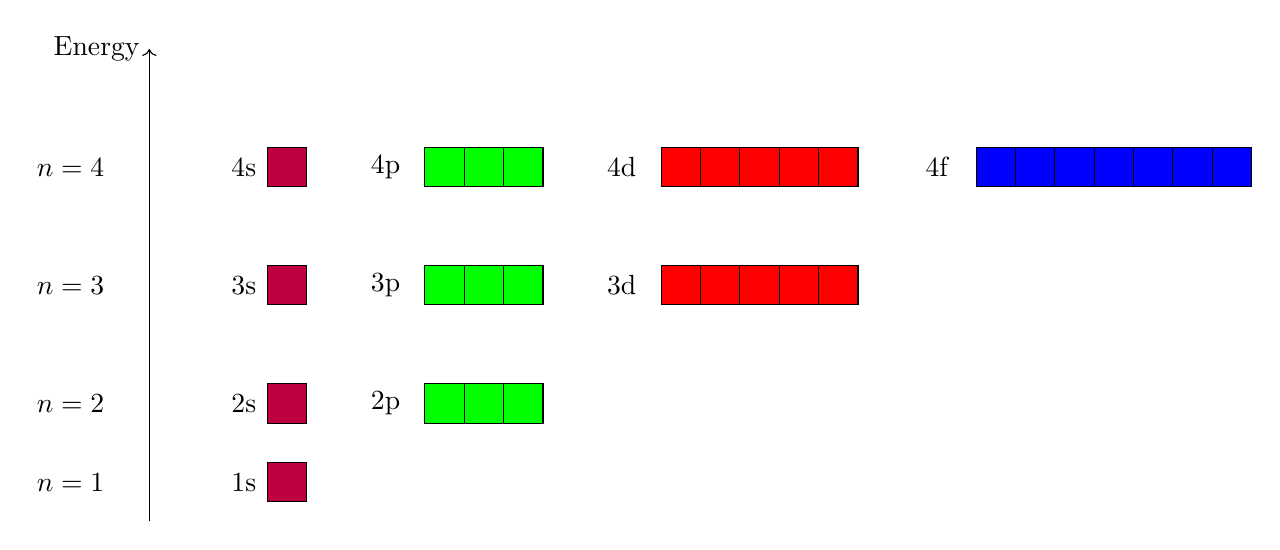
\begin{tikzpicture}

	% Energy axis
	\draw[->] (0,0) -- (0,6) node[left] {Energy};

	% n = 1
	\node at (-1,0.5) {\(n=1\)};
	\node at (1.2,0.5) {1s};
	\draw[fill=purple] (1.5,0.25) rectangle (2,0.75);

	% n = 2
	\node at (-1,1.5) {\(n=2\)};
	\node at (1.2,1.5) {2s};
	\draw[fill=purple] (1.5,1.25) rectangle (2,1.75);

	\node at (3,1.5) {2p};
	\foreach \i in {1,2,3} {
			\draw[fill=green] (3+\i*0.5,1.25) rectangle (3.5+\i*0.5,1.75);
		}

	% n = 3
	\node at (-1,3) {\(n=3\)};
	\node at (1.2,3) {3s};
	\draw[fill=purple] (1.5,2.75) rectangle (2,3.25);

	\node at (3,3) {3p};
	\foreach \i in {1,2,3} {
			\draw[fill=green] (3+\i*0.5,2.75) rectangle (3.5+\i*0.5,3.25);
		}

	\node at (6,3) {3d};
	\foreach \i in {1,2,3,4,5} {
			\draw[fill=red] (6+\i*0.5,2.75) rectangle (6.5+\i*0.5,3.25);
		}

	% n = 4
	\node at (-1,4.5) {\(n=4\)};
	\node at (1.2,4.5) {4s};
	\draw[fill=purple] (1.5,4.25) rectangle (2,4.75);

	\node at (3,4.5) {4p};
	\foreach \i in {1,2,3} {
			\draw[fill=green] (3+\i*0.5,4.25) rectangle (3.5+\i*0.5,4.75);
		}

	\node at (6,4.5) {4d};
	\foreach \i in {1,2,3,4,5} {
			\draw[fill=red] (6+\i*0.5,4.25) rectangle (6.5+\i*0.5,4.75);
		}

	\node at (10,4.5) {4f};
	\foreach \i in {1,2,3,4,5,6,7} {
			\draw[fill=blue] (10+\i*0.5,4.25) rectangle (10.5+\i*0.5,4.75);
		}

\end{tikzpicture}

\subsection*{Explanation}

The diagram represents the energy levels of atomic orbitals, arranged by the principal quantum number ($n$) and their corresponding subshells.

\begin{itemize}
	\item \textbf{Energy Axis:} The y-axis represents the increasing energy of the orbitals. As the energy increases, the orbitals are arranged vertically.
	\item \textbf{Principal Quantum Number ($n$):} Each horizontal row corresponds to a different value of $n$, the principal quantum number, representing different electron shells. For example:
	      \begin{itemize}
		      \item $n=1$: 1s orbital (lowest energy)
		      \item $n=2$: 2s and 2p orbitals
		      \item $n=3$: 3s, 3p, and 3d orbitals
		      \item $n=4$: 4s, 4p, 4d, and 4f orbitals (highest energy shown)
	      \end{itemize}
	      The value of $n$ corresponds to the shell and relates to the energy level and the row (period) in the periodic table.
	\item \textbf{Subshells and Orbitals:}
	      \begin{itemize}
		      \item \textbf{s-orbitals ($l=0$)} are spherical and represented by purple squares. They exist for each value of $n$ (1s, 2s, 3s, 4s).
		      \item \textbf{p-orbitals ($l=1$)} are dumbbell-shaped and represented by green squares. They appear starting from $n=2$ (2p, 3p, 4p) and have three possible orientations, corresponding to three green squares for each $p$-subshell.
		      \item \textbf{d-orbitals ($l=2$)} are more complex in shape and represented by red squares. They appear starting from $n=3$ (3d, 4d) and have five possible orientations, represented by five red squares for each $d$-subshell.
		      \item \textbf{f-orbitals ($l=3$)} are highly complex in shape and represented by blue squares. They appear starting from $n=4$ (4f) and have seven possible orientations, represented by seven blue squares for each $f$-subshell.
	      \end{itemize}
\end{itemize}

The horizontal arrangement of colored squares shows the degeneracy (number of orbitals) for each subshell, while the vertical arrangement corresponds to increasing energy.

\pagebreak

\subsection{Visualization of Electron Probability Density Functions and Orbitals}

% 1s Orbital
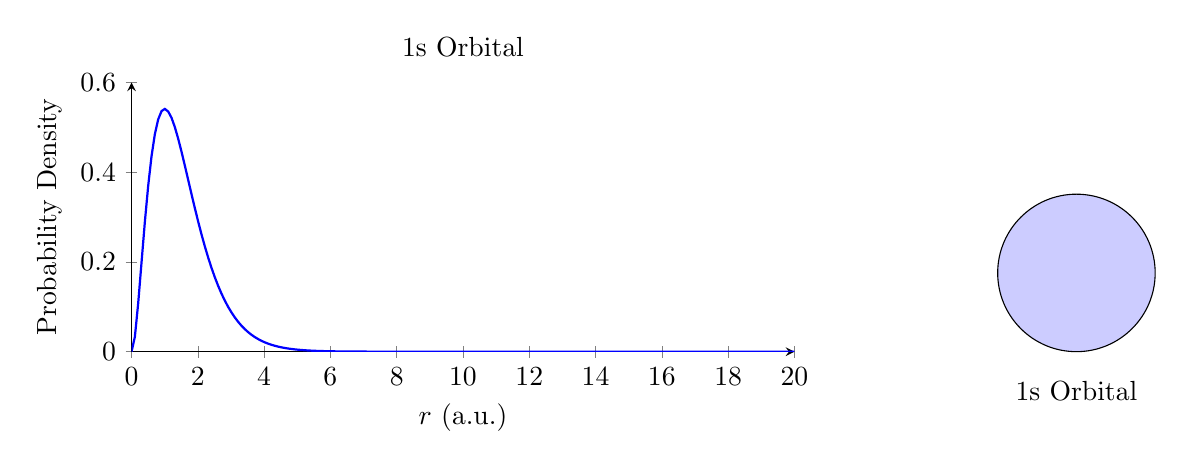
\begin{tikzpicture}
	% Plot for 1s orbital
	\begin{axis}[
			width=10cm,
			height=5cm,
			xmin=0, xmax=20,
			ymin=0, ymax=0.6,
			xlabel={$r$ (a.u.)},
			ylabel={Probability Density},
			axis x line=bottom,
			axis y line=left,
			title={1s Orbital}
		]
		\addplot [domain=0:20, samples=200, thick, blue] {4*(1)^3 * x^2 * exp(-2*x)};
	\end{axis}

	% 2D representation of 1s orbital
	\begin{scope}[shift={(12cm,1cm)}]
		\draw [fill=blue!20] (0,0) circle (1cm);
		\node at (0,-1.5) {1s Orbital};
	\end{scope}
\end{tikzpicture}

\vspace{1.5cm}

% 2s Orbital
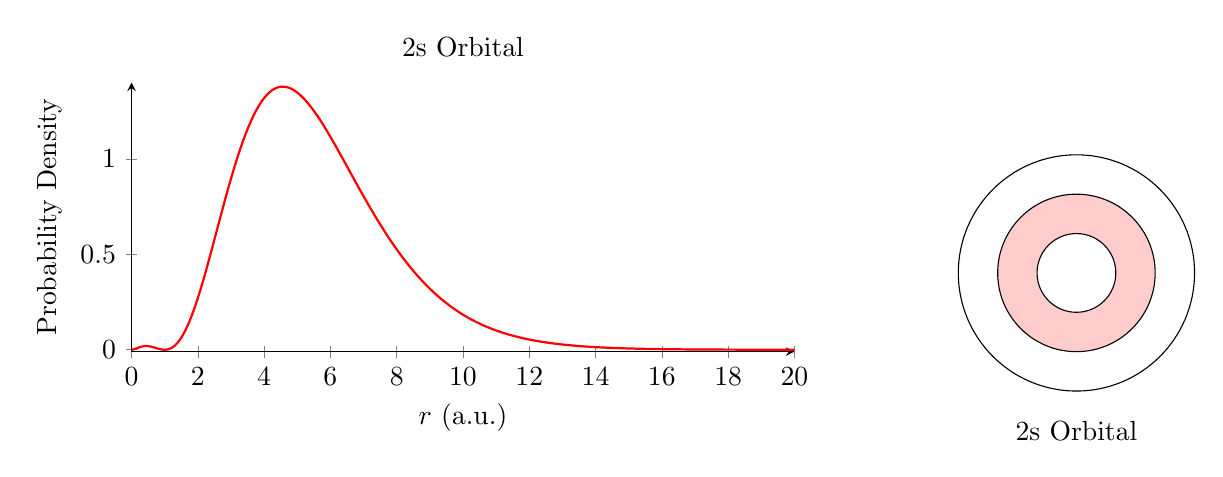
\begin{tikzpicture}
	% Plot for 2s orbital
	\begin{axis}[
			width=10cm,
			height=5cm,
			xmin=0, xmax=20,
			ymin=-0.01, ymax=1.4,
			xlabel={$r$ (a.u.)},
			ylabel={Probability Density},
			axis x line=bottom,
			axis y line=left,
			title={2s Orbital}
		]
		\addplot [domain=0:20, samples=200, thick, red] {(1/2)*(1)^3 * x^2 * (1 - x)^2 * exp(-x)};
	\end{axis}

	% 2D representation of 2s orbital
	\begin{scope}[shift={(12cm,1cm)}]
		\draw [fill=white] (0,0) circle (1.5cm);
		\draw [fill=red!20] (0,0) circle (1cm);
		\draw [fill=white] (0,0) circle (0.5cm);
		\node at (0,-2) {2s Orbital};
	\end{scope}
\end{tikzpicture}

\vspace{1.5cm}

% 2p Orbital
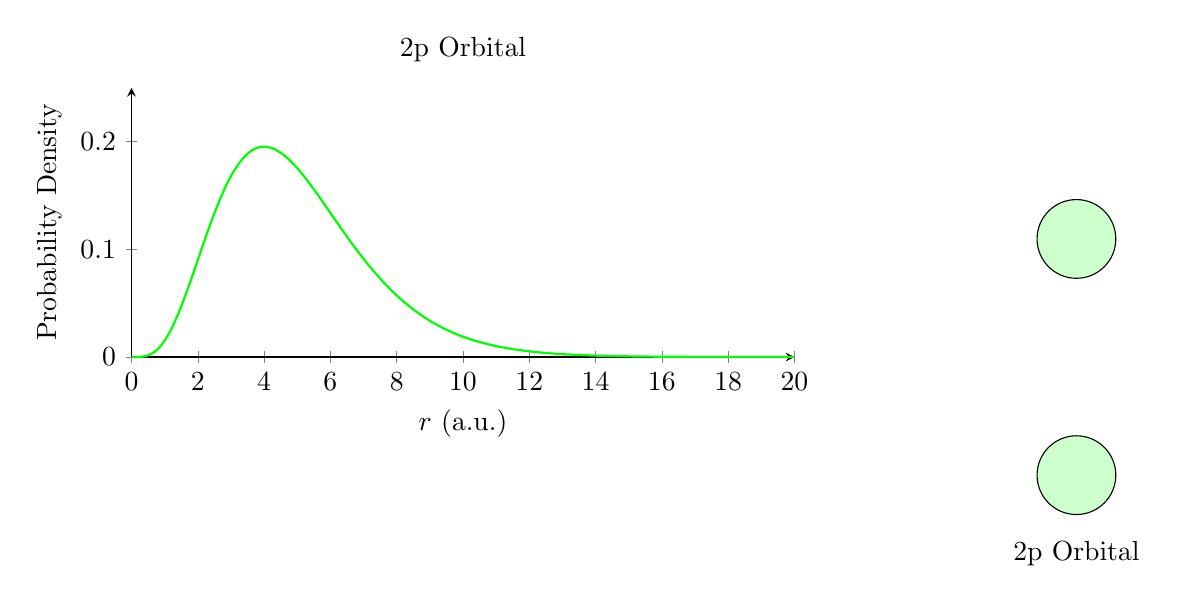
\begin{tikzpicture}
	% Plot for 2p orbital
	\begin{axis}[
			width=10cm,
			height=5cm,
			xmin=0, xmax=20,
			ymin=0, ymax=0.25,
			xlabel={$r$ (a.u.)},
			ylabel={Probability Density},
			axis x line=bottom,
			axis y line=left,
			title={2p Orbital}
		]
		\addplot [domain=0:20, samples=200, thick, green] {(1/24)*(1)^3 * x^4 * exp(-x)};
	\end{axis}

	% 2D representation of 2p orbital
	\begin{scope}[shift={(12cm,0)}]
		\draw [fill=green!20] (0,1.5) circle (0.5cm);
		\draw [fill=green!20] (0,-1.5) circle (0.5cm);
		\node at (0,-2.5) {2p Orbital};
	\end{scope}
\end{tikzpicture}

\section{Nature of Electrons}

Electrons exhibit wave-like properties, a fundamental concept in quantum mechanics. This wave nature is crucial in understanding atomic structure and electron behavior.

\subsection{Delocalization}

Delocalization occurs when we attempt to "measure" an electron. It describes an electron's wave that is not 3D localized.

\section{Atomic Structure}

\subsection{Electron Configuration}

The arrangement of electrons in an atom follows specific patterns:

\begin{align*}
	n & = 1: \quad 1s                            \\
	n & = 2: \quad 2s \quad 2p                   \\
	n & = 3: \quad 3s \quad 3p \quad 3d          \\
	n & = 4: \quad 4s \quad 4p \quad 4d \quad 4f
\end{align*}

Where $n$ represents the principal quantum number.

\section{Radial Probability}

The radial probability distribution shows the likelihood of finding an electron at a certain distance from the nucleus.

\begin{center}
	\begin{tikzpicture}
		\draw[->] (0,0) -- (4,0) node[right] {$r$};
		\draw[->] (0,0) -- (0,3) node[above] {$P(r)$};
		\draw[domain=0:3.8, smooth, variable=\x, blue] plot ({\x}, {2*\x*exp(-\x)});
		\node at (1.5,2.5) {1s};
		\draw[domain=0:3.8, smooth, variable=\x, red] plot ({\x}, {\x*\x*exp(-\x/2)});
		\node at (3,1.5) {2p};
	\end{tikzpicture}
\end{center}

This graph shows the radial probability distributions for 1s and 2p orbitals.

Shielding occurs when inner electrons partially shield outer electrons from the full nuclear charge. This leads to the concept of effective nuclear charge ($Z_{\text{eff}}$).


For outer core levels:
\[ 90\% \cdot (3-2) = 0.9 \quad \text{(eff)} \]

This means that .9 of the charge difference between the actual nuclear charge and the next lower noble gas configuration contributes to the effective nuclear charge.

For 2s, which is not shielded by 1s:
\[ 100\% \cdot (3-0) = 3 \]

The full charge difference contributes to $Z_{\text{eff}}$.

\section{Electron Configuration}

The arrangement of electrons in an atom follows the Aufbau principle, Pauli exclusion principle, and Hund's rule. The diagram below illustrates the order of filling orbitals:


\begin{center}
	\begin{tikzpicture}[scale=0.8]
		\draw[->] (0,0) -- (0,8) node[left] {Energy};
		\draw[->] (0,0) -- (8,0);

		\foreach \y/\l in {0.5/1s, 1.5/2s, 2/2p, 3/3s, 3.5/3p, 4/3d, 4.5/4s, 5/4p, 5.5/4d, 6/4f, 6.5/5s, 7/5p}
			{
				\node[left] at (0,\y) {\l};
				\draw[->] (0.2,\y) -- (1,\y);
			}

		\draw[->] (1.2,0.5) -- (1.2,1.5);
		\draw[->] (1.4,1.5) -- (1.4,2);
		\draw[->] (1.6,2) -- (1.6,3);
		\draw[->] (1.8,3) -- (1.8,3.5);
		\draw[->] (2,3.5) -- (2,4);
		\draw[->] (2.2,4) -- (2.2,4.5);
		\draw[->] (2.4,4.5) -- (2.4,5);
	\end{tikzpicture}
\end{center}

The full electron configuration for elements up to atomic number 87 (Francium) is:

\[ 1s^2 2s^2 2p^6 3s^2 3p^6 4s^2 3d^{10} 4p^6 5s^2 4d^{10} 5p^6 6s^2 4f^{14} 5d^{10} 6p^6 7s^2 5f^{14} \]

\subsection{Example Configurations}

\textbf{Sodium}
\[ \text{Sodium} \rightarrow 1s^2 2s^2 2p^6 3s^1 \rightarrow [\text{Ne}] 3s^1 \]

\textbf{Argon}
\[ \text{Argon} \rightarrow 1s^2 2s^2 2p^6 3s^2 3p^6 \rightarrow [\text{Ne}] 3s^2 3p^6 \rightarrow [\text{Ar}] \]

\section{Quantum Numbers}

For the principal quantum number $n = 3$:

\begin{itemize}
	\item $\ell = \{s=0, p=1, d=2, f=3...\}$
	\item $m_\ell = -\ell, ..., 0, ..., +\ell$
	\item $m_s = -\frac{1}{2}, +\frac{1}{2}$
\end{itemize}

\section{Hund's Rule}

Hund's rule states that electrons in degenerate orbitals (same energy) will occupy different orbitals with the same spin before pairing up. For example, in the $2p$ orbital:

\[ (2p_x \uparrow, 2p_y \uparrow, 2p_z \uparrow) \text{ is preferred over } (2p_x \uparrow\downarrow, 2p_y, 2p_z) \]

This configuration has $m_s = +\frac{1}{2}$ for each unpaired electron.

\section{Molecular Orbital Theory}

Molecular Orbital (MO) theory explains the electronic structure of molecules by considering the combination of atomic orbitals (AOs) into molecular orbitals. These molecular orbitals extend over the entire molecule and can hold electrons from multiple atoms. MO theory provides a more accurate understanding of the bonding and antibonding interactions in a molecule compared to Valence Bond Theory.

\subsection{Potential Energy of Hydrogen Molecule}

\begin{center}
	\includegraphics[width=0.7\textwidth]{1.png}
\end{center}
\textit{Schematic representation of the potential energy of two hydrogen atoms as a function of the distance between them. As distance decreases, the potential energy reaches a minimum value of $-458$ kJ mol$^{-1}$ at a distance of $0.74$ Å. The value of $D_0$ for $H_2$ is 432 kJ mol$^{-1}$ or 4.48 eV molecule$^{-1}$.}

The graph above highlights the potential energy curve for the interaction between two hydrogen atoms. The minimum point represents the equilibrium bond length, $R_e$, where the potential energy is at its lowest and most stable. The depth of the well, $D_e$, reflects the bond dissociation energy, and it illustrates the energy required to break the bond and separate the atoms to infinity.

\textbf{Bond Energy and Stability:}
\begin{itemize}
	\item $R_e$: The equilibrium bond length where attractive and repulsive forces balance.
	\item $D_0$: The dissociation energy that corresponds to the strength of the bond between hydrogen atoms.
	\item The deeper the well in the graph, the stronger the bond between atoms.
\end{itemize}

In the context of Molecular Orbital Theory, the bonding molecular orbital (MO) formed from the constructive interference of atomic orbitals leads to the stabilization and energy minimization observed at $R_e$. On the other hand, destructive interference can lead to an antibonding orbital, which increases the potential energy as $R_{AB}$ approaches zero.

\subsection{Electron Probability Density in H$_2$ Molecule}

The electron probability density in a molecule is crucial to understanding the behavior of molecular orbitals. In MO theory, electrons are not confined to individual atoms but are distributed over the entire molecule. The following figure illustrates the probability density for finding an electron in the H$_2$ molecule at three different internuclear distances.

\begin{center}
	\includegraphics[width=0.7\textwidth]{2.png}
\end{center}
\textit{The probability density for finding an electron in the H$_2$ molecule, plotted at three internuclear distances: (a) 8a$_0$, (b) 3.5a$_0$, and (c) 1.4a$_0$. At the equilibrium bond length (c), a significant buildup of electron density between the nuclei is visible.}

This diagram shows three different stages of electron probability density as two hydrogen atoms approach each other:

\begin{enumerate}
	\item \textbf{Large Separation (8a$_0$) - No Interaction:}
	      At large distances, as shown in (a), the two hydrogen atoms do not interact, and the electron densities remain localized around each nucleus. This represents a situation where the atomic orbitals are too far apart to overlap.

	\item \textbf{Constructive Interference Begins (3.5a$_0$):}
	      As the atoms move closer, as shown in (b), constructive interference between the atomic orbitals begins. This is the first sign of bond formation as electron density starts to accumulate between the nuclei. This constructive overlap is essential in forming bonding molecular orbitals, which results in the lowering of energy and the stabilization of the molecule.

	\item \textbf{H$_2$ at Equilibrium Bond Length (1.4a$_0$):}
	      At the equilibrium bond length, illustrated in (c), the overlap of the atomic orbitals is maximal, leading to significant electron density between the nuclei. This concentration of electron density between the two hydrogen atoms is what holds them together in a covalent bond. The bonding molecular orbital created by this overlap has a lower energy than the individual atomic orbitals, contributing to the stability of the H$_2$ molecule.
\end{enumerate}

\textbf{Key Points to Note:}


\begin{itemize}

	\item As the hydrogen atoms approach one another, the electron density starts to build between the nuclei due to constructive interference, forming a bonding molecular orbital.
	\item At the equilibrium bond length, this bonding interaction is at its strongest, resulting in the maximum overlap of atomic orbitals.
	\item The behavior of the electron density between the atoms is a direct consequence of quantum mechanical principles that govern molecular orbital formation.

\end{itemize}

In the case of H$_2$, both electrons occupy the bonding molecular orbital, leading to the observed covalent bond. This distribution of electron density provides a qualitative understanding of why the molecule is stable at this bond length.

\subsection{Bonding and Antibonding Molecular Orbitals of H$_2$}

In MO theory, the combination of atomic orbitals (AOs) can result in the formation of either bonding or antibonding molecular orbitals (MOs). The following figure depicts the wave functions and electron densities for the H$_2$ molecule, illustrating the bonding and antibonding interactions along the internuclear axis.

\begin{center}
	\includegraphics[width=0.7\textwidth]{3.png}
\end{center}
\textit{Antibonding and bonding molecular orbitals of H$_2$ along the internuclear axis in the linear combination of atomic orbitals (LCAO) approximation. The bonding orbital shows increased probability density between the nuclei, while the antibonding orbital shows decreased probability density.}

The diagram above presents a comparison between:

\begin{itemize}
	\item The independent atomic orbitals (non-interacting case)
	\item Bonding molecular orbitals ($\sigma_{g1s}$)
	\item Antibonding molecular orbitals ($\sigma^*_{u1s}$)
\end{itemize}
In MO theory, atomic orbitals combine based on the principles of constructive and destructive interference:

\begin{itemize}
	\item \textbf{Non-interacting Orbitals:}
	      When the atoms are far apart and non-interacting, the electron density is localized around each nucleus. The wave functions, shown in the bottom row, remain independent and do not show any overlap. The electron density is confined to each atom.

	\item \textbf{Bonding Orbitals:}
	      Constructive interference of the wave functions from atomic orbitals leads to the formation of a bonding orbital. In this case, the wave functions ($\sigma_{g1s}$) combine additively, leading to an increased electron density between the two nuclei, as illustrated in the middle row. This increased electron density stabilizes the molecule, lowering its energy.

	\item \textbf{Antibonding Orbitals:}
	      Destructive interference results in the formation of antibonding orbitals ($\sigma^*_{u1s}$). The wave functions subtract from each other, leading to a node between the nuclei where electron density is reduced to zero, as shown in the top row. This decrease in electron density destabilizes the molecule and raises its energy.
\end{itemize}

\textbf{Key Features:}

\begin{itemize}

	\item In the bonding orbital, the electron probability density ($\sigma_{{g1s}^2}$) is concentrated between the nuclei, facilitating covalent bonding.
	\item In contrast, the antibonding orbital ($\sigma^{*}_{{u1s}^2}$) shows a significant decrease in electron density between the nuclei, resulting in repulsion and higher energy.
	\item The molecular orbital approximation allows us to predict the relative stability of molecules. Bonding orbitals lower the total energy, while antibonding orbitals raise it.

\end{itemize}


The balance between the population of bonding and antibonding orbitals determines the overall stability of the H$_2$ molecule. In stable molecules, bonding orbitals are filled, and antibonding orbitals remain unfilled.

\subsection{Graphical Representation of Bonding and Antibonding MOs}

In Molecular Orbital theory, the combination of atomic orbitals (AOs) can lead to the formation of bonding or antibonding molecular orbitals depending on whether the interference is constructive or destructive. The following figure shows a graphical representation of these combinations.

\begin{center}
	\includegraphics[width=0.7\textwidth]{4.png}
\end{center}
\textit{Graphical representation of the linear combination of atomic orbitals (AOs) resulting in a bonding molecular orbital (a) and an antibonding molecular orbital (b). The black dots show the approximate positions of the nuclei.}

\begin{itemize}
	\item In \textbf{(a)}, constructive interference between the AOs leads to the formation of a bonding molecular orbital ($\sigma_{g1s}$), where electron density is concentrated between the nuclei, stabilizing the molecule.

	\item In \textbf{(b)}, destructive interference results in an antibonding molecular orbital ($\sigma^*_{u1s}$), where electron density is reduced between the nuclei, leading to destabilization.

	\item The positions of the nuclei are represented by the black dots, emphasizing that electron density is more concentrated between the nuclei in bonding orbitals, while in antibonding orbitals, it is concentrated outside the internuclear region.
\end{itemize}

These graphical representations highlight the qualitative differences in electron distribution between bonding and antibonding molecular orbitals.

\subsection{Correlation Diagrams for First-Period Diatomic Molecules}

Molecular orbitals for diatomic molecules are constructed from the atomic orbitals of each atom. The following diagrams show the energy correlation for different molecules, starting with H$_2^+$, H$_2$, and He$_2^+$.

\begin{center}
	\begin{minipage}{0.32\textwidth}
		\centering
		\includegraphics[width=0.9\textwidth]{5.1.png}
		\textit{Correlation diagram for H$_2^+$ in the LCAO approximation. The bonding orbital is stabilized relative to the noninteracting system. $E_{1s} + (-\Delta E) = E_{\sigma g1s}$, so $\Delta E$ is a positive number.}
	\end{minipage}
	\begin{minipage}{0.32\textwidth}
		\centering
		\includegraphics[width=0.9\textwidth]{5.2.png}
		\textit{Correlation diagram for H$_2$ in the LCAO approximation. The blue arrows indicate electron filling in accordance with the Aufbau principle.}
	\end{minipage}
	\begin{minipage}{0.32\textwidth}
		\centering
		\includegraphics[width=0.9\textwidth]{5.3.png}
		\textit{Correlation diagram for He$_2^+$. The additional electron in the antibonding orbital reduces the bond order compared with that in H$_2$.}
	\end{minipage}
\end{center}

\textbf{Key Points:}
\begin{itemize}
	\item In H$_2^+$, the bonding orbital is stabilized by the energy difference $-\Delta E$.
	\item For H$_2$, the bonding orbital $\sigma_{g1s}$ is filled by two electrons, leading to bond formation.
	\item In He$_2^+$, an additional electron occupies the antibonding orbital $\sigma^*_{u1s}$, reducing the bond order and making the bond weaker than in H$_2$.
\end{itemize}

\subsection{Table: Electron Configurations and Bond Orders for First-Row Diatomic Molecules}

\begin{center}
	\includegraphics[width=0.7\textwidth]{5.4.png}
\end{center}
\textit{Electron configurations and bond orders for first-row diatomic molecules. This table summarizes the electron configurations, bond orders, bond energies, and bond lengths for H$_2^+$, H$_2$, He$_2^+$, and He$_2$.}

From the table, we can observe:
\begin{itemize}
	\item H$_2^+$ has a bond order of $\frac{1}{2}$ with bond energy 255 kJ mol$^{-1}$ and bond length of 1.06 Å.
	\item H$_2$ has a bond order of 1, with a bond energy of 431 kJ mol$^{-1}$ and bond length of 0.74 Å.
	\item He$_2^+$ has a bond order of $\frac{1}{2}$, a bond energy of 251 kJ mol$^{-1}$, and bond length of 1.08 Å.
	\item He$_2$ has a bond order of 0, indicating no stable bond between two helium atoms.
\end{itemize}

\subsection{Correlation Diagrams and Molecular Orbitals for Second-Period Diatomic Molecules}

For second-period diatomic molecules, the molecular orbitals (MOs) are constructed from the atomic orbitals of the constituent atoms, including the $2s$ and $2p$ orbitals. The following figure shows the correlation diagrams and the molecular orbitals for N$_2$ and F$_2$.

\begin{center}
	\includegraphics[width=0.7\textwidth]{6.png}
\end{center}
\textit{Correlation diagrams and molecular orbitals for second-period diatomic molecules. (a) Correlation diagram and molecular orbitals calculated for N$_2$. (b) Correlation diagram and molecular orbitals calculated for F$_2$.}

\textbf{Key Points:}
\begin{itemize}
	\item In the case of N$_2$, where $Z \leq 7$, the $\pi_{2p}$ orbitals are lower in energy than the $\sigma_{2p_z}$ orbital. The filling of bonding orbitals ($\sigma_{2s}$, $\sigma^*_{2s}$, $\pi_{2p_x}$, $\pi_{2p_y}$, $\sigma_{2p_z}$) leads to a strong triple bond.

	\item For F$_2$, with $Z \geq 8$, the $\sigma_{2p_z}$ orbital is lower in energy than the $\pi_{2p_x}$ and $\pi_{2p_y}$ orbitals. The addition of electrons to the antibonding orbitals ($\pi^*_{2p_x}$, $\pi^*_{2p_y}$, $\sigma^*_{2p_z}$) weakens the bond, resulting in a single bond.

	\item The diagrams also show the molecular orbital isosurfaces, which enclose the regions of highest electron density. Red and blue areas represent the positive and negative phases of the wave function, showing nodal planes where the wave function changes sign.
\end{itemize}

\textbf{Bonding in N$_2$:}
\begin{itemize}
	\item The bond order is 3, as there are six bonding electrons and no electrons in antibonding $\pi^*_{2p}$ orbitals.
	\item This leads to a very strong and stable triple bond in N$_2$.
\end{itemize}

\textbf{Bonding in F$_2$:}
\begin{itemize}
	\item The bond order is 1, as two bonding electrons are canceled by two electrons in antibonding orbitals ($\pi^*_{2p_x}$ and $\pi^*_{2p_y}$).
	\item This results in a much weaker single bond compared to N$_2$.
\end{itemize}

This diagram emphasizes the energy ordering of orbitals and how electron filling impacts bond strength in second-period diatomic molecules.

\subsection{Correlation Diagram for Heteronuclear Diatomic Molecules}

Heteronuclear diatomic molecules consist of two atoms with different electronegativities. In such molecules, the atomic orbitals of the more electronegative atom (B) are lower in energy compared to those of atom A. The diagram below shows the correlation diagram and orbital filling for boron monoxide (BO).

\begin{center}
	\includegraphics[width=0.7\textwidth]{7.png}
\end{center}
\textit{Correlation diagram for heteronuclear diatomic molecules, AB. The atomic orbitals for the more electronegative atom (B) are displaced downward because they have lower energies than those for A. The orbital filling shown is for boron monoxide (BO).}

\textbf{Key Features:}
\begin{itemize}
	\item In heteronuclear diatomic molecules, the atomic orbitals of the more electronegative atom (B) are lower in energy. This causes an asymmetry in the molecular orbitals' energy levels.

	\item The $\sigma_{2p_z}$ orbital, formed from the combination of $2p$ orbitals of both atoms, is lower in energy compared to the $\pi_{2p_x}$ and $\pi_{2p_y}$ orbitals, as seen in BO.

	\item The bonding orbitals are filled following the Aufbau principle. In this case, bonding occurs in the $\sigma_{2p_z}$, $\pi_{2p_x}$, and $\pi_{2p_y}$ orbitals, while antibonding occurs in the $\sigma^*_{2s}$ and $\pi^*_{2p_x}$, $\pi^*_{2p_y}$ orbitals.

	\item Due to the energy disparity between the atoms' orbitals, the contributions of each atom to the bonding molecular orbitals are unequal, with the more electronegative atom (B) contributing more to the lower-energy bonding orbitals.
\end{itemize}

\textbf{Bonding in BO:}
\begin{itemize}
	\item The orbital filling diagram shows that bonding occurs primarily in the $\pi$ orbitals and the $\sigma_{2p_z}$ orbital.
	\item The bond order is determined by the number of bonding and antibonding electrons, and in the case of BO, there is significant bonding between the two atoms due to the partially filled bonding orbitals.
\end{itemize}

Heteronuclear diatomic molecules often exhibit polar bonds due to the difference in electronegativity, which further affects the molecular properties.

\subsection{Paramagnetic and Diamagnetic}

In chemistry and physics, \textbf{paramagnetic} and \textbf{diamagnetic} refer to the magnetic properties of atoms or molecules:

\begin{itemize}
	\item \textbf{Paramagnetic}: Paramagnetic substances have unpaired electrons, which give rise to a magnetic moment. When an external magnetic field is applied, these unpaired electrons align with the field, causing the material to be weakly attracted to it. This effect is temporary; once the field is removed, the magnetic alignment disappears. Examples include oxygen (\(\text{O}_2\)) and ions with unpaired electrons, such as \(\text{Fe}^{3+}\) and \(\text{Mn}^{2+}\).
	\item \textbf{Diamagnetic}: Diamagnetic substances have all electrons paired, resulting in no permanent magnetic moment. These substances are slightly repelled by an external magnetic field, and this repulsion is also temporary. Examples include nitrogen (\(\text{N}_2\)) and most organic compounds.
\end{itemize}

Paramagnetic and diamagnetic properties are essential in fields like magnetic resonance imaging (MRI) and magnetic material design, where the behavior of materials in magnetic fields is crucial.

\subsection{Bond Length}

\textbf{Bond length} is the distance between the nuclei of two bonded atoms in a molecule. It depends on various factors, including:

\begin{itemize}
	\item \textbf{Bond Order}: Higher bond orders (e.g., double or triple bonds) typically result in shorter bond lengths due to the stronger attraction between atoms.
	\item \textbf{Atomic Size}: Larger atoms tend to form longer bonds since their electron clouds are more spread out.
	\item \textbf{Electron Distribution}: Bonding versus antibonding electron populations influence bond length. Electrons in bonding orbitals shorten the bond, while electrons in antibonding orbitals lengthen it.
	\item \textbf{Resonance and Delocalization}: In molecules with delocalized electrons, such as benzene, bond lengths may be intermediate between those typical for single and double bonds.
\end{itemize}

Understanding bond length is important in determining molecular shape, strength of bonds, and reactivity in chemical reactions.

\chapter{Gasses}

\section{Introduction to Gases}
Gases are a state of matter characterized by their lack of fixed shape or volume. Gas particles are in constant, rapid motion and are spaced far apart compared to the particles in solids or liquids. Here are some fundamental properties of gases:

\begin{itemize}
	\item \textbf{No Significant Intermolecular Forces:} In an ideal gas, particles are assumed to have no significant intermolecular forces between them. This means that gas particles neither attract nor repel each other, allowing them to move independently. This assumption simplifies gas behavior, especially under low-pressure and high-temperature conditions.

	\item \textbf{Pressure and Collisions:} Gas pressure is primarily caused by collisions between gas particles and the walls of their container. The force exerted by these collisions per unit area defines the pressure of the gas. In an ideal gas, we assume elastic collisions, meaning the total kinetic energy of particles remains constant.
\end{itemize}

\section{Boyle's Law}
Boyle's Law states that the pressure \( P \) of a given amount of gas is inversely proportional to its volume \( V \), at constant temperature:
\[
	P \propto \frac{1}{V} \quad \text{or} \quad PV = \text{constant}.
\]

\noindent \textbf{Explanation:} As the volume of a gas decreases, particles have less space to move, resulting in more frequent collisions with the container walls, which increases pressure. Conversely, increasing the volume decreases the frequency of collisions, lowering the pressure.

\begin{figure}[h]
	\centering
	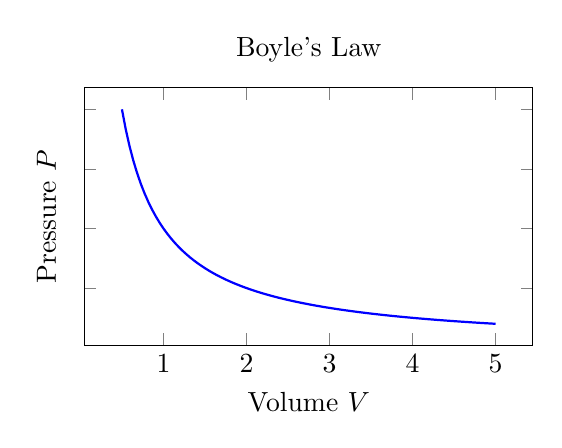
\begin{tikzpicture}
		\begin{axis}[
				xlabel={Volume \( V \)},
				ylabel={Pressure \( P \)},
				domain=0.5:5,
				samples=100,
				width=0.6\textwidth,
				height=0.4\textwidth,
				title={Boyle's Law},
				yticklabels={,,}
			]
			\addplot[blue, thick] {1/x};
		\end{axis}
	\end{tikzpicture}
	\caption{Graph of Boyle's Law showing the inverse relationship between pressure and volume.}
\end{figure}

\section{Non-Uniform Collisions and Energy Distribution}
The collisions between gas particles are non-uniform, meaning not all particles collide with the same energy. This variability in collision energy results in an uneven distribution of kinetic energy among gas particles, leading to what is known as the Maxwell-Boltzmann distribution of speeds.

\section{Charles's Law}
Charles's Law states that the volume \( V \) of a gas is directly proportional to its absolute temperature \( T \) when pressure is kept constant:
\[
	\frac{V}{T} = \text{constant}.
\]

\noindent \textbf{Explanation:} When the temperature of a gas increases, the kinetic energy of the gas particles also increases, causing them to collide with greater force and frequency. To maintain constant pressure, the volume of the gas must increase to allow particles more space.

\begin{figure}[h]
	\centering
	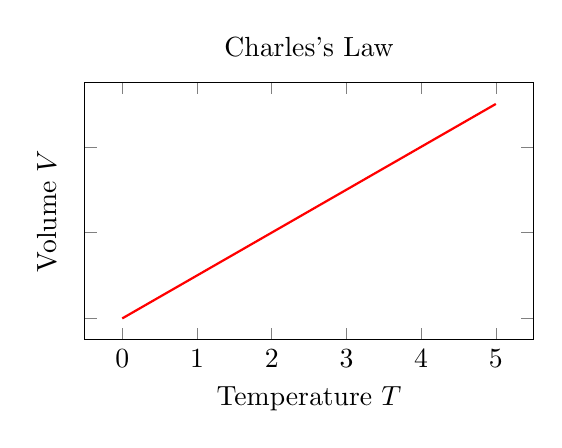
\begin{tikzpicture}
		\begin{axis}[
				xlabel={Temperature \( T \)},
				ylabel={Volume \( V \)},
				domain=0:5,
				samples=100,
				width=0.6\textwidth,
				height=0.4\textwidth,
				title={Charles's Law},
				yticklabels={,,}
			]
			\addplot[red, thick] {x};
		\end{axis}
	\end{tikzpicture}
	\caption{Graph of Charles's Law showing the direct relationship between volume and temperature (in Kelvin).}
\end{figure}

\section{Absolute Zero and the Kelvin Scale}
Absolute zero, defined as \(-273.15^\circ\text{C}\), is the lowest possible temperature at which particles theoretically have no kinetic energy. This point serves as the foundation of the Kelvin temperature scale, where \(0 \, \text{K}\) is absolute zero. The Kelvin scale is widely used in gas law calculations because it provides a direct measure of thermal energy.

\section{Avogadro's Law}
Avogadro's Law states that the volume \( V \) of a gas is directly proportional to the number of moles \( n \) of gas present, provided temperature and pressure are constant:
\[
	V \propto n \quad \text{or} \quad \frac{V}{n} = \text{constant}.
\]

\noindent \textbf{Explanation:} Increasing the amount of gas (number of moles) at constant temperature and pressure will increase the volume, as there are more particles that need space to move.

\begin{figure}[h]
	\centering
	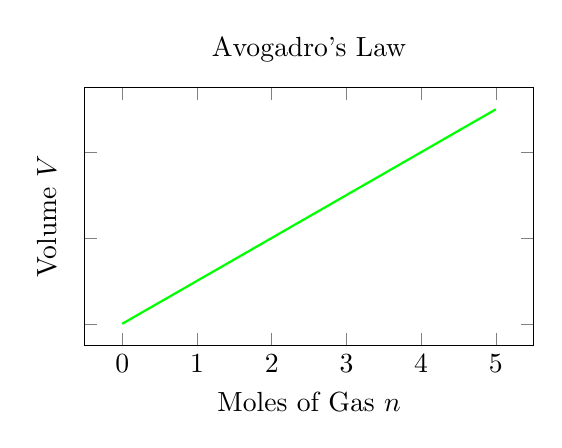
\begin{tikzpicture}
		\begin{axis}[
				xlabel={Moles of Gas \( n \)},
				ylabel={Volume \( V \)},
				domain=0:5,
				samples=100,
				width=0.6\textwidth,
				height=0.4\textwidth,
				title={Avogadro's Law},
				yticklabels={,,}
			]
			\addplot[green, thick] {x};
		\end{axis}
	\end{tikzpicture}
	\caption{Graph of Avogadro's Law showing the direct relationship between volume and the amount of gas in moles.}
\end{figure}

\section{Summary of Gas Laws}
\dfn{Ideal Gas Law}{
	The behavior of gases can be summarized by the Ideal Gas Law, which combines Boyle's, Charles's, and Avogadro's laws:
	\[
		PV = nRT,
	\]
	where \begin{itemize}
		\item \( P \) is the pressure of the gas,
		\item \( V \) is the volume of the gas,
		\item \( n \) is the amount of substance (in moles),
		\item \( R \) is the ideal gas constant,
		\item \( T \) is the temperature (in Kelvin).
	\end{itemize}

}


\subsection{Units for Each Variable}
To use the Ideal Gas Law correctly, we need to ensure all variables are in consistent units:
\begin{itemize}
	\item \( P \) (Pressure): Measured in atmospheres (atm), pascals (Pa), or torr. For simplicity, we'll use atmospheres, where \(1 \, \text{atm} = 101{,}325 \, \text{Pa}\).
	\item \( V \) (Volume): Measured in liters (L) or cubic meters (m³), where \(1 \, \text{L} = 0.001 \, \text{m}^3\).
	\item \( n \) (Moles): Measured in moles (mol).
	\item \( R \) (Ideal Gas Constant): Varies depending on the pressure and volume units. Common values are:
	      \begin{itemize}
		      \item \( R = 0.0821 \, \text{L atm} \cdot \text{K}^{-1} \cdot \text{mol}^{-1} \),
		      \item \( R = 8.314 \, \text{J} \cdot \text{K}^{-1} \cdot \text{mol}^{-1} \).
	      \end{itemize}
	\item \( T \) (Temperature): Measured in Kelvin (K). To convert from Celsius to Kelvin, use \( T(K) = T(°\text{C}) + 273.15 \).
\end{itemize}

\subsection{General Gas Equation}
For conditions where gases do not behave ideally, we may use the General Gas Equation, also known as the Combined Gas Law, which combines Boyle's, Charles's, and Gay-Lussac's laws:
\[
	\frac{P_1 V_1}{T_1} = \frac{P_2 V_2}{T_2}.
\]
This equation describes the relationship between pressure, volume, and temperature of a gas when transitioning between two states, where:
\begin{itemize}
	\item \( P_1 \) and \( P_2 \) are the initial and final pressures,
	\item \( V_1 \) and \( V_2 \) are the initial and final volumes,
	\item \( T_1 \) and \( T_2 \) are the initial and final temperatures (in Kelvin).
\end{itemize}

\ex{Ideal Gas Law Example}{
	Suppose we want to find the volume of \( 1.5 \) moles of an ideal gas at a pressure of \( 2.0 \) atm and a temperature of \( 300 \) K.

	Given:
	\[
		P = 2.0 \, \text{atm}, \quad n = 1.5 \, \text{mol}, \quad T = 300 \, \text{K}, \quad R = 0.0821 \, \text{L atm} \cdot \text{K}^{-1} \cdot \text{mol}^{-1}.
	\]

	Using the Ideal Gas Law:
	\[
		PV = nRT.
	\]

	Solving for \( V \):
	\[
		V = \frac{nRT}{P}.
	\]

	Substitute the values:
	\[
		V = \frac{(1.5 \, \text{mol})(0.0821 \, \text{L atm} \cdot \text{K}^{-1} \cdot \text{mol}^{-1})(300 \, \text{K})}{2.0 \, \text{atm}}.
	\]

	Calculating each part:
	\[
		V = \frac{1.5 \times 0.0821 \times 300}{2.0} = \frac{36.945}{2.0} = 18.4725 \, \text{L}.
	\]

	Thus, the volume of the gas is approximately \( 18.47 \, \text{L} \). This example illustrates the importance of using consistent units to ensure accurate calculations when applying the Ideal Gas Law.
}

\subsection{Conversion Between mmHg and Pa}

To convert between millimeters of mercury (mmHg) and pascals (Pa), we use the following relationship:
\[
	1 \, \text{mmHg} = 133.322 \, \text{Pa}.
\]

To convert a pressure \( P \) in mmHg to Pa, multiply by \( 133.322 \):
\[
	P(\text{Pa}) = P(\text{mmHg}) \times 133.322.
\]

\ex{Example Conversion from mmHg to Pa}{
	Suppose we have a pressure of \( 760 \, \text{mmHg} \). To convert to Pa:
	\[
		P(\text{Pa}) = 760 \, \text{mmHg} \times 133.322 = 101{,}325.72 \, \text{Pa}.
	\]
	Thus, \( 760 \, \text{mmHg} \) is approximately \( 101{,}325 \, \text{Pa} \), which is close to standard atmospheric pressure.
}

\section{Mixtures of Gases}

When dealing with mixtures of gases, we can treat the system as if there were a single gas by using the total amount \( n = n_{\text{total}} \).

\subsection{Dalton's Law of Partial Pressures}

Dalton's Law of Partial Pressures states that the total pressure exerted by a mixture of non-reacting gases is equal to the sum of the partial pressures of the individual gases. Mathematically, this can be expressed as:
\[
	P_{\text{tot}} = P_1 + P_2 + \dots
\]
where \( P_{\text{tot}} \) is the total pressure and \( P_1, P_2, \dots \) are the partial pressures of each gas in the mixture.

Each partial pressure \( P_i \) is the pressure that each gas would exert if it were alone in the container at the same temperature and volume.

\ex{Calculating the Pressure of a Gas Mixture}{
	Suppose we have a mixture of \( 1 \, \text{g} \) of hydrogen (\( \text{H}_2 \)) and \( 5 \, \text{g} \) of helium (\( \text{He} \)) in a container. We can calculate the partial pressures of each gas and the total pressure.

	\begin{enumerate}
		\item First, calculate the number of moles of each gas:
		      \[
			      n_{\text{H}_2} = \frac{1}{2.02} = 0.495 \, \text{mol}, \quad n_{\text{He}} = \frac{5}{4.003} = 1.25 \, \text{mol}.
		      \]

		\item The total number of moles is:
		      \[
			      n_{\text{total}} = n_{\text{H}_2} + n_{\text{He}} = 0.495 + 1.25 = 1.745 \, \text{mol}.
		      \]

		\item Using the Ideal Gas Law, the total pressure \( P_{\text{tot}} \) is given by:
		      \[
			      P_{\text{tot}} = \frac{n_{\text{total}} R T}{V}.
		      \]
	\end{enumerate}
}

\subsection{Mole Fraction and Partial Pressure}

The mole fraction \( x_i \) of each gas in the mixture is the ratio of the number of moles of that gas to the total number of moles:
\[
	x_i = \frac{n_i}{n_{\text{total}}}.
\]

The partial pressure \( P_i \) of each gas can then be calculated using the mole fraction and the total pressure:
\[
	P_i = x_i \cdot P_{\text{tot}}.
\]

\ex{Calculating Mole Fractions and Partial Pressures}{
	Given the previous example with \( n_{\text{H}_2} = 0.495 \, \text{mol} \) and \( n_{\text{He}} = 1.25 \, \text{mol} \):

	\begin{enumerate}
		\item The mole fraction of hydrogen is:
		      \[
			      x_{\text{H}_2} = \frac{n_{\text{H}_2}}{n_{\text{total}}} = \frac{0.495}{1.745} \approx 0.284.
		      \]

		\item The mole fraction of helium is:
		      \[
			      x_{\text{He}} = \frac{n_{\text{He}}}{n_{\text{total}}} = \frac{1.25}{1.745} \approx 0.716.
		      \]

		\item If the total pressure \( P_{\text{tot}} \) is known, the partial pressures can be calculated as:
		      \[
			      P_{\text{H}_2} = x_{\text{H}_2} \cdot P_{\text{tot}}, \quad P_{\text{He}} = x_{\text{He}} \cdot P_{\text{tot}}.
		      \]
	\end{enumerate}
}

\section{Gases: Van der Waals Equation}

The Van der Waals equation is an adjustment to the ideal gas law that accounts for the non-ideal behavior of real gases. Unlike ideal gases, real gases have finite volumes and intermolecular forces, which the Van der Waals equation incorporates through two constants: \( a \) and \( b \).

\begin{equation}
	P = \frac{RT}{V - b} - \frac{a}{V^2}
\end{equation}

where:
\begin{itemize}
	\item \( P \): Pressure of the gas
	\item \( V \): Volume of the gas
	\item \( T \): Temperature in Kelvin
	\item \( R \): Universal gas constant
	\item \( a \): Constant representing intermolecular attraction
	\item \( b \): Constant representing the finite volume occupied by gas molecules
\end{itemize}

\subsection{Properties}

\begin{itemize}
	\item \textbf{Volume Reduction (V is reduced by a constant \( b \)):} \\
	      The constant \( b \) accounts for the finite volume of gas molecules. Unlike in an ideal gas, where molecules are considered to have negligible size, real gas molecules occupy space. Therefore, the effective volume available for molecular movement is reduced by \( b \), which is proportional to the size of the molecules. The adjusted volume is \( V - b \), indicating that the actual space for movement is less than the total volume.

	      \begin{itemize}
		      \item \textit{Meaning:} The presence of \( b \) acknowledges that molecules have a physical volume, which reduces the space in which they can freely move.
	      \end{itemize}

	\item \textbf{Pressure Increase (P is increased by a constant \( a \), divided by \( V^2 \)):} \\
	      The constant \( a \) represents the attraction between gas molecules. In an ideal gas, it is assumed that molecules do not interact. However, in real gases, molecules attract each other, which slightly reduces the force with which they collide with the container walls, thus reducing the pressure. To correct for this, the term \( \frac{a}{V^2} \) is added to the equation, increasing the calculated pressure to account for these attractive forces.

	      \begin{itemize}
		      \item \textit{Meaning:} The presence of \( a \) reflects the attractive forces between molecules, which tend to draw them closer together, effectively increasing the pressure when intermolecular attractions are taken into account.
	      \end{itemize}

	\item \textbf{Interpretation of Constant \( b \):} \\
	      The constant \( b \) is related to the repulsion between molecules due to their electron clouds. When molecules are close together, the repulsive forces caused by overlapping electron clouds prevent them from occupying the same space, which effectively increases the volume each molecule occupies.

	\item \textbf{Interpretation of Constant \( a \):} \\
	      The constant \( a \) represents the strength of attractive forces between molecules, which are particularly significant at low temperatures and high pressures. These attractions arise from forces such as Van der Waals forces, which can cause the molecules to cluster together. This attraction reduces the pressure exerted on the container walls.

	\item \textbf{Microscopic Interpretation of \( a \):} \\
	      On a microscopic level, the attractive forces symbolized by \( a \) manifest as weak interactions, like dipole-dipole interactions, London dispersion forces, and hydrogen bonding. These forces cause molecules to momentarily attract each other, especially when they are in close proximity, reducing their kinetic impact on the walls and, hence, the pressure.
\end{itemize}

\subsection{Summary of Van der Waals Equation Adjustments}

The Van der Waals equation modifies the ideal gas law to better represent real gases:
\[
	P = \frac{RT}{V - b} - \frac{a}{V^2}
\]
where:
\begin{itemize}
	\item The volume term \( V - b \) corrects for the finite size of molecules.
	\item The pressure term \( \frac{a}{V^2} \) corrects for intermolecular attractions.
\end{itemize}

These adjustments allow the equation to describe real gas behavior more accurately than the ideal gas law, especially under conditions where gases are compressed (high pressure) or at low temperatures, where deviations from ideal behavior are most significant.

\section{Intermolecular Forces: London Dispersion Forces}

London dispersion forces are a type of weak intermolecular force that occurs due to the temporary fluctuations in the electron distribution around atoms or molecules. These forces play a significant role in the attraction between nonpolar molecules, and their strength increases with the size and electron cloud of the molecule.

\subsection{Mechanism of London Dispersion Forces}

\begin{itemize}
	\item \textbf{Distortion of Electron Clouds:} \\
	      When atoms or molecules come close to each other, the electron clouds around them can be distorted. This distortion occurs because electrons are not fixed in place; they can move within their atomic or molecular orbitals. Due to this mobility, electrons may become more concentrated on one side of an atom or molecule than the other.

	      \begin{itemize}
		      \item \textit{Result:} This uneven electron distribution creates a temporary separation of charge, where one side becomes slightly more negative and the opposite side slightly more positive.
	      \end{itemize}

	\item \textbf{Formation of an Instantaneous Dipole:} \\
	      The distortion of the electron cloud results in an \textit{instantaneous dipole}. This means that, at any given moment, the molecule has a temporary separation of positive and negative charges. This dipole is not permanent; it forms due to the random movement of electrons and may change or disappear as the electrons continue to move.

	      \begin{itemize}
		      \item \textit{Meaning:} The instantaneous dipole represents a momentary charge separation, which is a key feature of London dispersion forces.
	      \end{itemize}

	\item \textbf{Induction of Dipoles in Neighboring Molecules:} \\
	      The presence of an instantaneous dipole in one atom or molecule can influence neighboring molecules. The partially positive or negative side of the dipole can attract or repel the electrons in a nearby atom or molecule, creating an \textit{induced dipole}.

	      \begin{itemize}
		      \item \textit{Explanation:} The initial dipole induces a similar dipole in the neighboring molecule, which in turn induces dipoles in other nearby molecules, leading to a cascading effect.
	      \end{itemize}

	\item \textbf{Attractive Interactions between Dipoles:} \\
	      The induced dipoles in neighboring atoms or molecules interact with each other. Although these dipoles are temporary, they align such that the partial positive end of one molecule is attracted to the partial negative end of another, resulting in a weak net attraction. This attraction, though weak, is sufficient to hold nonpolar molecules together under certain conditions.

	      \begin{itemize}
		      \item \textit{Outcome:} The interaction between these temporary dipoles is responsible for London dispersion forces, a significant intermolecular force in nonpolar compounds.
	      \end{itemize}
\end{itemize}

\subsection{Summary of London Dispersion Forces}

\begin{itemize}
	\item London dispersion forces arise from temporary fluctuations in electron distribution within atoms or molecules.
	\item They involve the formation of instantaneous dipoles, which induce dipoles in nearby molecules.
	\item The dipoles interact to create a weak attraction, which can stabilize nonpolar molecules and atoms in close proximity.
	\item These forces become stronger with increasing atomic or molecular size, as larger electron clouds are more easily distorted.
\end{itemize}

\begin{center}
	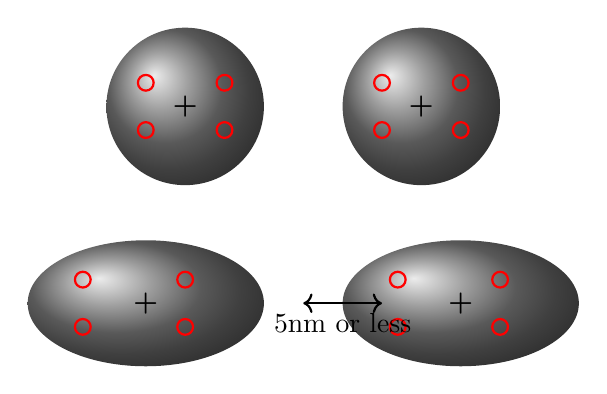
\begin{tikzpicture}

		% Top row - Simple atoms
		% Left atom
		\shade[ball color=gray] (0,1.5) circle (1); % Atom 1
		\node at (0,1.5) {\textbf{+}}; % Positive nucleus
		\foreach \x in {-0.5, 0.5} {
				\foreach \y in {0.3, -0.3} {
						\draw[red, thick] (\x,1.5+\y) circle (0.1); % Electron clouds
					}
			}

		% Right atom
		\shade[ball color=gray] (3,1.5) circle (1); % Atom 2
		\node at (3,1.5) {\textbf{+}}; % Positive nucleus
		\foreach \x in {-0.5, 0.5} {
				\foreach \y in {0.3, -0.3} {
						\draw[red, thick] (3+\x,1.5+\y) circle (0.1); % Electron clouds
					}
			}

		% Bottom row - Interacting atoms with elongated shapes
		% Left atom (elongated)
		\shade[ball color=gray] (-0.5,-1) ellipse (1.5 and 0.8); % Atom 3
		\node at (-0.5,-1) {\textbf{+}}; % Positive nucleus
		\foreach \x in {-0.8, 0.5} {
				\foreach \y in {0.3, -0.3} {
						\draw[red, thick] (\x-0.5,-1+\y) circle (0.1); % Electron clouds
					}
			}

		% Right atom (elongated)
		\shade[ball color=gray] (3.5,-1) ellipse (1.5 and 0.8); % Atom 4
		\node at (3.5,-1) {\textbf{+}}; % Positive nucleus
		\foreach \x in {-0.8, 0.5} {
				\foreach \y in {0.3, -0.3} {
						\draw[red, thick] (3.5+\x,-1+\y) circle (0.1); % Electron clouds
					}
			}

		% Distance label
		\draw[<->, thick] (1.5,-1) -- (2.5,-1);
		\node[below] at (2,-1) {5nm or less};

	\end{tikzpicture}
\end{center}

\section{Intermolecular Forces: Dipole-Dipole Interactions}

Dipole-dipole interactions occur between polar molecules, where there is a permanent separation of charge due to differences in electronegativity between atoms within the molecule. These interactions are stronger than London dispersion forces because they involve permanent dipoles rather than temporary ones.

\subsection{Formation of Dipoles}

\begin{itemize}
	\item \textbf{Electronegativity Differences and Molecular Asymmetry:} \\
	      In a polar molecule, atoms with different electronegativities are bonded together. The more electronegative atom attracts the bonding electrons more strongly, creating a partial negative charge, while the less electronegative atom has a partial positive charge. This separation of charges leads to a permanent dipole.

	      \begin{itemize}
		      \item \textit{Example:} In a molecule like chloromethane (\ce{CH3Cl}), the chlorine atom is more electronegative than carbon and hydrogen, causing an uneven electron distribution. The result is a partial negative charge on the chlorine and a partial positive charge on the hydrogens, creating a permanent dipole.
	      \end{itemize}

	\item \textbf{Dipole Orientation:} \\
	      For a dipole-dipole interaction to occur, the dipoles must not cancel out geometrically. The orientation and structure of the molecule should allow for a net dipole moment. This interaction between permanent dipoles causes attraction between polar molecules, as the positive end of one molecule is attracted to the negative end of another.

\end{itemize}

\subsection{Strength of Dipole-Dipole Interactions}

\begin{itemize}
	\item \textbf{Permanent vs. Induced Dipoles:} \\
	      Permanent dipoles, such as those found in polar molecules, are stronger than induced dipoles, which arise in nonpolar molecules through London dispersion forces. Permanent dipoles create a lasting separation of charge, leading to more stable and stronger interactions between molecules.

	\item \textbf{Inducing Additional Dipoles:} \\
	      Even though they are stronger, permanent dipoles can also induce dipoles in neighboring nonpolar molecules through the process of dipole-induced dipole interactions, similar to how instantaneous dipoles induce neighboring dipoles.

\end{itemize}

\subsection{Combined Intermolecular Forces}

Molecules with dipole-dipole interactions also experience London dispersion forces. While dipole-dipole interactions arise from permanent dipoles, London dispersion forces are present in all molecules due to temporary fluctuations in electron distribution. Therefore, polar molecules with permanent dipoles benefit from the additive effect of both forces.

\begin{center}
	\begin{tikzpicture}

		% Molecule 1 - Dipole in CH3Cl
		\node (C1) at (0,0) {C};
		\node[right=0.5cm of C1] (H1) {H};
		\node[above left=0.7cm and 0.4cm of C1] (Cl1) {Cl};
		\node[below left=0.7cm and 0.4cm of C1] (H2) {H};
		\draw[->, thick] (C1) -- (Cl1); % Dipole from C to Cl
		\node[above right=0.3cm and 0.6cm of C1] {\small $\delta^+$};
		\node[above left=0.4cm and 0.3cm of Cl1] {\small $\delta^-$};

		% Molecule 2 - Dipole in neighboring CH3Cl
		\node (C2) at (3,0) {C};
		\node[right=0.5cm of C2] (H3) {H};
		\node[above left=0.7cm and 0.4cm of C2] (Cl2) {Cl};
		\node[below left=0.7cm and 0.4cm of C2] (H4) {H};
		\draw[->, thick] (C2) -- (Cl2); % Dipole from C to Cl
		\node[above right=0.3cm and 0.6cm of C2] {\small $\delta^+$};
		\node[above left=0.4cm and 0.3cm of Cl2] {\small $\delta^-$};

		% Arrow showing dipole-dipole attraction
		\draw[<->, dashed, thick] (Cl1) -- (C2);

	\end{tikzpicture}
\end{center}

\textit{Diagram of two \ce{CH3Cl} molecules showing dipole-dipole interaction. The dipole moment points from the carbon atom to the more electronegative chlorine atom, leading to attraction between the molecules.}

\section{Gases at the Microscopic Level}

\subsection{Key Characteristics of Gases}
\begin{enumerate}
	\item \textbf{Molecules collide with other molecules and walls:} \\
	      Gas molecules are in constant, random motion and frequently collide with each other and the walls of their container. These collisions create pressure as the molecules exert force on the container walls.

	\item \textbf{Elastic collisions:} \\
	      The collisions between gas molecules are elastic, meaning there is no net loss of kinetic energy. This ensures the total kinetic energy of the system remains constant in the absence of external influences.

	\item \textbf{Distance between molecules $\gg$ size of molecules:} \\
	      The average distance between gas molecules is much greater than the size of the molecules themselves. This property allows gases to be compressible and enables them to spread out to fill the container they occupy.

	\item \textbf{No intermolecular interactions:} \\
	      In an ideal gas, we assume there are no attractive or repulsive forces between molecules except during collisions. This assumption is valid at low pressures and high temperatures when the molecules are far apart.

	\item \textbf{Kinetic energy proportional to temperature ($\bar{E} \propto T$):} \\
	      The average kinetic energy of gas molecules is directly proportional to the absolute temperature. As temperature increases, the speed and kinetic energy of the molecules also increase.
\end{enumerate}

\subsection{Forces Associated with Molecular Collisions}
\begin{itemize}
	\item \textbf{Translational kinetic energy ($\frac{1}{2}mv^2$):} \\
	      The kinetic energy of gas molecules depends on their mass ($m$) and speed ($v$). The expression $\frac{1}{2}mv^2$ describes this energy.

	\item \textbf{Frequency of collisions:} \\
	      The rate of collisions depends on the number of molecules, their velocity, and the space in which they move.

	\item \textbf{Impulse ($\Delta p = m \Delta v$):} \\
	      Collisions result in changes in momentum, where impulse is defined as the product of mass and change in velocity.
\end{itemize}

\section{Gas Kinetic Theory and Related Concepts}

\subsection{Pressure and Molecular Speeds}
\begin{itemize}
	\item Pressure ($P$) is proportional to the number density ($\frac{n}{V}$) and the mean square speed of molecules ($\overline{u^2}$):
	      \[
		      P \propto \frac{n}{V} \overline{u^2}
	      \]
	      However, not all molecules have the same speed. The distribution of speeds can be represented using a Maxwell-Boltzmann distribution, which shows how the velocities of molecules vary at different temperatures.

	\item Graphs of speed distributions at different temperatures:
	      \begin{itemize}
		      \item At higher temperatures (e.g., 1000 K vs. 300 K), the curve flattens and shifts to the right, indicating a broader range of speeds and higher average velocity.
		      \item The area under each curve represents the total number of molecules, which remains constant.
	      \end{itemize}

	\item The mean square speed ($\overline{u^2}$) is calculated as:
	      \[
		      \overline{u^2} = \frac{1}{i} \sum_{n=1}^{i} u_n^2
	      \]

	\item Since pressure acts equally in all directions (e.g., $x$, $y$, $z$), we use a $\frac{1}{3}$ factor:
	      \[
		      P = \frac{1}{3} \frac{Nm \overline{u^2}}{V}
	      \]
\end{itemize}

\subsection{Ideal Gas Law and Molecular Kinetic Energy}
\begin{itemize}
	\item The ideal gas law can be expressed as:
	      \[
		      PV = \frac{1}{3} Nm \overline{u^2}
	      \]

	\item Relating this to the kinetic theory:
	      \[
		      \overline{u^2} = \frac{3kT}{m}
	      \]

	\item The root mean square speed ($u_{rms}$) of the molecules:
	      \[
		      u_{rms} = \sqrt{\overline{u^2}} = \sqrt{\frac{3kT}{m}}
	      \]

	\item The average kinetic energy ($\overline{E_k}$) of a gas molecule:
	      \[
		      \overline{E_k} = \frac{3}{2} kT
	      \]
	      where $k$ is Boltzmann's constant.
\end{itemize}

\subsection{Temperature and Kinetic Energy}
\begin{itemize}
	\item Temperature is directly proportional to the average kinetic energy:
	      \[
		      T \propto \overline{E_k}
	      \]

	\item The relationship between average kinetic energy, temperature, and number of molecules:
	      \[
		      \overline{E_k} = \frac{3}{2} \frac{k}{N_A} T
	      \]
	      where $N_A$ is Avogadro's number.
\end{itemize}

\subsection{Diffusion and Effusion}
\begin{itemize}
	\item \textbf{Diffusion} refers to the process of gas molecules spreading out due to random motion.

	\item \textbf{Effusion} is the escape of gas molecules through a small hole into a vacuum.

	\item The rate of effusion follows Graham's law:
	      \[
		      \frac{A}{B} = \sqrt{\frac{M_B}{M_A}}
	      \]
	      where $M_A$ and $M_B$ are the molar masses of gases $A$ and $B$, respectively.
\end{itemize}

\section{Van der Waals Equation for Real Gases}

The Van der Waals equation is a modification of the ideal gas law, created to account for the non-ideal behavior of real gases. This equation introduces two main corrections to the ideal gas assumptions: the excluded volume and intermolecular forces.

\subsection{Excluded Volume Correction}
In the ideal gas law, gas molecules are assumed to occupy no space. However, in reality, molecules have a finite volume, which affects the actual volume available for gas movement. The equation for the ideal gas volume can be approximated as:
\[
	V_{\text{ideal}} = V_{\text{container}} - V_{\text{molecules}} \approx V_{\text{container}} - bn
\]
where:
\begin{itemize}
	\item \( V_{\text{container}} \) is the total volume of the container.
	\item \( V_{\text{molecules}} = bn \), where \( b \) is a constant that represents the volume occupied by one mole of gas molecules, and \( n \) is the number of moles.
\end{itemize}
Thus, the available volume for the gas is slightly less than the container volume due to the excluded volume of the molecules.

\begin{center}
	\textit{Intuition:} Think of it as the ``crowdedness'' effect. When gas molecules occupy space, there's less free volume for them to move around, especially in smaller containers or at higher pressures.
\end{center}

\subsection{Intermolecular Forces Correction:}
In an ideal gas, it is assumed that there are no interactions between molecules. However, real gas molecules experience attractive forces, which can affect the pressure exerted on the walls of the container. The Van der Waals equation adjusts for this by modifying the pressure term as follows:
\[
	\left( P + a \left( \frac{n}{V} \right)^2 \right)
\]
where:
\begin{itemize}
	\item \( P \) is the observed pressure.
	\item \( a \) is a constant specific to each gas, representing the strength of intermolecular attractions.
	\item \( \frac{n}{V} \) is the concentration of gas molecules.
\end{itemize}
The term \( a \left( \frac{n}{V} \right)^2 \) is added to the pressure to account for attractive forces between gas molecules, effectively increasing the pressure to balance these forces.

\begin{center}
	\textit{Intuition:} At low pressures and large volumes, these attractions are minimal. However, as molecules come closer (e.g., at higher pressures), the attractions become significant, reducing the effective pressure.
\end{center}

\subsection{The Van der Waals Equation:}
Combining these corrections, the Van der Waals equation is written as:
\[
	\left( P + a \left( \frac{n}{V} \right)^2 \right) (V - bn) = nRT
\]
where \( R \) is the gas constant and \( T \) is the temperature. This equation provides a more accurate representation of gas behavior under various conditions, especially at high pressures and low volumes.

\section{Mean Free Path and Collision Frequency}

\subsection{Mean Free Path (\(\lambda\))}
\dfn{Mean Free Path}{
	\((\lambda)\) represents the average distance a molecule travels before colliding with another molecule. This concept is crucial in kinetic theory, as it helps us understand how molecules move in a gas and how often they interact.
}

\ex{Formula Derivation}{
	\begin{itemize}
		\item \(\lambda \propto \frac{1}{d^2}\): The mean free path is inversely proportional to the square of the diameter (\(d\)) of the molecules. This means that larger molecules (greater \(d\)) will have a shorter mean free path, as they are more likely to collide.
		\item \(\lambda \propto \frac{1}{(N/V) \, d^2}\): Taking into account the number of molecules per unit volume \((N/V)\) and the molecular diameter \((d^2)\), the mean free path also becomes inversely proportional to the density of molecules and their size.
	\end{itemize}
}

\ex{Final Formula for \(\lambda\)}{
	\[
		\lambda = \frac{RT}{(\sqrt{2}) \pi d^2 P N_A}
	\]
	where:
	\begin{itemize}
		\item \(R\) is the gas constant,
		\item \(T\) is the temperature,
		\item \(P\) is the pressure,
		\item \(N_A\) is Avogadro's number.
	\end{itemize}

	This formula shows that the mean free path is also affected by temperature and pressure. \textit{Higher temperatures increase \(\lambda\)} (since molecules move faster and may spread out more), while \textit{higher pressures decrease \(\lambda\)} (as molecules are packed closer together).
}

\ex{Example Calculation for Helium (He)}{
	For Helium (He), with:
	\begin{itemize}
		\item \(d = 210 \, \text{pm}\) (picometers),
		\item \(T = 150 \, \text{K}\),
		\item \(P = 1 \, \text{atm}\) (1 bar or \(10^5 \, \text{Pa}\)),
	\end{itemize}
	we can calculate:
	\[
		\lambda \approx 1.06 \times 10^5 \, \text{pm}
	\]
}

\subsection{Collision Frequency}
\dfn{Collision frequency}{ is the number of collisions a molecule undergoes per second. It’s an important parameter in understanding how quickly molecules interact in a gas.}

\ex{Formula for Collision Frequency}{
	The collision frequency can be calculated using:
	\[
		\text{Collision Frequency} = \text{speed} \times \frac{1}{\text{mean free path}}
	\]
	This is because the frequency of collisions depends on how fast molecules are moving and how far they travel between collisions.
}

\ex{Example Calculation}{
	Given a \textit{molecular speed of 967 m/s} and a mean free path of \(1.06 \times 10^{-7} \, \text{m}\), the collision frequency is:
	\[
		\frac{967 \, \text{m/s}}{1.06 \times 10^{-7} \, \text{m}} \approx 9.12 \times 10^9 \, \text{collisions/second}
	\]
	This high frequency shows that even though molecules travel relatively far between collisions (in the context of their small size), they still undergo a vast number of collisions per second due to their high speeds.
}

\subsection{Intuition and Practical Insight}
\begin{itemize}
	\item \textbf{Mean Free Path}: A longer mean free path indicates fewer collisions, which can happen in a low-pressure gas where molecules are spaced further apart. In contrast, a short mean free path, as found in high-pressure gases, means molecules are densely packed and collide frequently.
	\item \textbf{Collision Frequency}: This value gives insight into the level of molecular interaction. High collision frequencies suggest gases are behaving more like a dense fluid, with molecules constantly interacting. This is significant in processes like diffusion, heat conduction, and viscosity in gases.
\end{itemize}

By breaking down these concepts and using real-world examples, it becomes easier to connect theoretical formulas with tangible properties of gases.

\section{Solids, Liquids, and Phase Transitions}

This section explores key concepts in thermodynamics related to phase transitions, specific heat capacity, and the energy changes involved in state changes.

\subsection{Specific Heat Capacity}
The specific heat capacity, \( C_p \), is a measure of the energy required to raise the temperature of a substance. It is defined as:
\[
C_p = \frac{q_p}{T}
\]
where:
\begin{itemize}
    \item \( q_p \) is the heat added at constant pressure.
    \item \( T \) is the temperature.
\end{itemize}

Alternatively, the relationship can be expressed in terms of enthalpy (\( \Delta H \)):
\[
q_p = \Delta H \quad \Rightarrow \quad C_p = \frac{\Delta H}{\Delta T} \quad \text{or} \quad \Delta H = m \, c \, \Delta T
\]
where \( m \) is the mass and \( c \) is the specific heat capacity.

\subsection{Enthalpy and Energy Changes}
Enthalpy change (\( \Delta H \)) is associated with heat added or removed from a system. The enthalpy change can be written as:
\[
\Delta H = E + PV
\]
where:
\begin{itemize}
    \item \( E \) represents the internal energy of the system.
    \item \( PV \) is the work done by the system due to pressure and volume.
\end{itemize}

\begin{center}
    \textit{Insight:} Added energy can either change the state of a substance (latent heat) or increase its kinetic energy (translational, rotational, or vibrational motion), contributing to a temperature change.
\end{center}

\subsection{Phase Transitions and Molecular Motion}
Different phases (solid, liquid, and gas) exhibit distinct types of molecular motion and arrangements:
\begin{center}
    \begin{tabular}{|c|c|c|c|c|}
        \hline
        \textbf{Phase} & \textbf{Translation} & \textbf{Rotation} & \textbf{Vibration} & \textbf{Intermolecular Distance} \\
        \hline
        Solid & None & None & About fixed position & Short, fixed \\
        \hline
        Liquid & Limited & Hindered & Free & Short, dynamic \\
        \hline
        Gas & Free & Free & Free & Long, variable \\
        \hline
    \end{tabular}
\end{center}

\subsection{Endothermic and Exothermic Processes}
\begin{itemize}
    \item \textbf{Endothermic processes:} The products are at a higher energy level than the reactants. Examples include melting and vaporization, where energy is absorbed.
    \item \textbf{Exothermic processes:} The opposite of endothermic, these processes release energy as products form from reactants.
\end{itemize}

\subsection{Comparing Heat of Fusion and Heat of Vaporization}
The heat of fusion (\( \Delta H_{\text{fusion}} \)) is generally much smaller than the heat of vaporization (\( \Delta H_{\text{vaporization}} \)). This is because:
\[
\Delta H_{\text{fusion}} \ll \Delta H_{\text{vaporization}}
\]
\begin{center}
    \textit{Insight:} Fusion only partially disrupts intermolecular forces, while vaporization requires breaking most intermolecular forces, leading to a significantly higher energy requirement.
\end{center}

\subsection{Heating Curve and Phase Changes}
A heating curve illustrates how temperature changes over time as heat is added to a substance. During phase transitions (such as melting and boiling), temperature remains constant while energy is absorbed to change the phase.

\begin{figure}[h!]
    \centering
    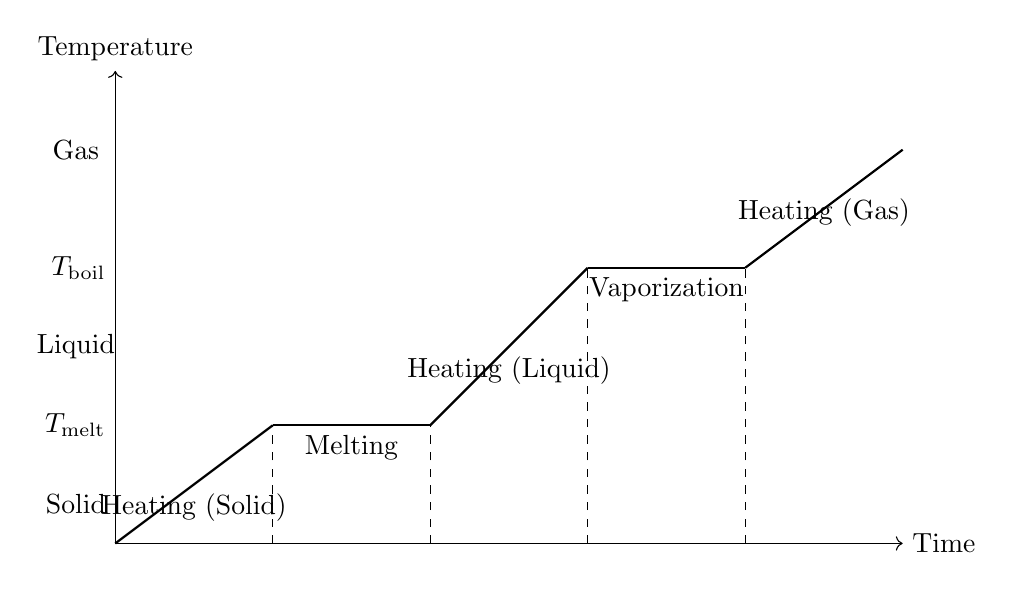
\begin{tikzpicture}
        % Axes
        \draw[->] (0,0) -- (10,0) node[right] {Time};
        \draw[->] (0,0) -- (0,6) node[above] {Temperature};

        % Labels
        \node at (-0.5,0.5) {Solid};
        \node at (-0.5,2.5) {Liquid};
        \node at (-0.5,5.0) {Gas};

        % Temperature vs. Time lines
        % Phase 1: Heating Solid
        \draw[thick] (0,0) -- (2,1.5);
        \node[below] at (1,0.75) {Heating (Solid)};

        % Phase 2: Melting (constant temperature)
        \draw[thick] (2,1.5) -- (4,1.5);
        \node[below] at (3,1.5) {Melting};

        % Phase 3: Heating Liquid
        \draw[thick] (4,1.5) -- (6,3.5);
        \node[below] at (5,2.5) {Heating (Liquid)};

        % Phase 4: Vaporization (constant temperature)
        \draw[thick] (6,3.5) -- (8,3.5);
        \node[below] at (7,3.5) {Vaporization};

        % Phase 5: Heating Gas
        \draw[thick] (8,3.5) -- (10,5);
        \node[below] at (9,4.5) {Heating (Gas)};

        % Dotted Lines to indicate phase transitions
        \draw[dashed] (2,0) -- (2,1.5);
        \draw[dashed] (4,0) -- (4,1.5);
        \draw[dashed] (6,0) -- (6,3.5);
        \draw[dashed] (8,0) -- (8,3.5);

        % Temperature Labels
        \node[left] at (0,1.5) {$T_{\text{melt}}$};
        \node[left] at (0,3.5) {$T_{\text{boil}}$};
    \end{tikzpicture}
    \caption{Heating Curve showing temperature changes during phase transitions.}
\end{figure}

\end{document}